\documentclass[dvipsnames,table]{include/thesisclass}
% Main File - Based on thesisclass.cls
% Comments are mostly in English
% ------------------------------------------------------------------------------
% Further files in folder:
%  - include/cmds.tex (for macros and additional commands)
%  - include/kitlogo.pdf (for titlepage)
%  - lit.bib (bibtex bibliography database)
%  - include/titlepage.tex (for layout of titelpage)
% ------------------------------------------------------------------------------
% Useful Supplied Packages:
% amsmath, amssymb, mathtools, bbm, upgreek, nicefrac,
% siunitx, varioref, booktabs, graphicx, tikz, multicol
%\usepackage[dvipsnames,table]{xcolor}
\usepackage{media9}

\usepackage{listings}
%images
%\usepackage{graphicx}
\usepackage{float}
\usepackage{pdfpages}
\usepackage{subcaption}



%for tables
\usepackage{tabularx}
\usepackage{dcolumn,booktabs}
\renewcommand\thempfootnote{\arabic{mpfootnote}} %to show footnote with numbers in tables
\newcolumntype{d}[1]{D{.}{.}{#1}}
\newcommand\mc[1]{\multicolumn{1}{c}{#1}} % handy shortcut macro

% acronyms
\usepackage{acronym} 


%misc
\usepackage{siunitx}
\usepackage{glossaries}
\usepackage{trfsigns}
\usepackage{enumitem}
\newcommand{\thz}{\SI{}{\tera \hertz}}

%tikz & pgfplots
\usepackage{tikz,tikzscale,pgfplots,pgfplotstable,circuitikz, tikz-timing}
\usetikzlibrary{arrows,shapes,shadows,external,decorations.pathmorphing}
\tikzexternalize[optimize=false,prefix=tikz/]
\usetikztiminglibrary{arrows}

\usepgfplotslibrary{units,fillbetween,colormaps} 
\pgfplotsset{compat=newest}

\pgfdeclarehorizontalshading{visiblelight}{50bp}{
	color(0.00000000000000bp)=(violet);
	color(8.33333333333333bp)=(blue);
	color(16.66666666666670bp)=(cyan);
	color(25.00000000000000bp)=(green);
	color(33.33333333333330bp)=(yellow);
	color(41.66666666666670bp)=(orange);
	color(50.00000000000000bp)=(red)
} 







%\usepackage{tikz-palattice}

%% -------------------------
%% |    Thesis Settings    |
%% -------------------------
% english or ngerman (new german für neue deutsche Rechtschreibung statt german)
\SelectLanguage{english}
% details on this thesis
\newcommand{\thesisauthor}{Olena Manzhura}
\newcommand{\thesisentopic}{A Terabit sampling system with a photonics time-stretch ADC}
%\newcommand{\thesisentopic}{Ein Terabit Abtastsystem mit Photonic-Time-Stretch Analog-Digital-Wandler}
\newcommand{\thesislongtopic}{}
\newcommand{\thesisinstitute}{Institute for Data Processing and Electronics (IPE)}
\newcommand{\thesisreviewerone}{Prof. Dr. Anke-Susanne Müller (LAS)}
\newcommand{\thesisreviewertwo}{Dr. Michele Caselle (IPE)}
\newcommand{\thesisadvisorone}{} % to use: enter names and uncomment in titlepg
\newcommand{\thesisadvisortwo}{}
\newcommand{\thesistimestart}{15.11.2020} % on titlepage
\newcommand{\thesistimeend}{13.08.2021} % on titlepage
\newcommand{\thesistimehandin}{13.08.2021} % on second page 'preamble'
\newcommand{\thesispagehead}{Master Thesis: \thesisentopic} % page heading





%% ---------------------
%% |    PDF - Setup    |
%% ---------------------
% This information will appear embed into the PDF file as meta data, but will 
% not be printed anywhere
\hypersetup
{
    pdfauthor={\thesisauthor},
    pdftitle={Masterarbeit: \thesisentopic},
    pdfsubject={\thesislongtopic},
    pdfkeywords={kit,etit,master,thesis,\thesisauthor}
}



%% --------------------------------------
%% |    Settings for Word Separation    |
%% --------------------------------------
% Help for separation:
% In German package the following hints are additionally available:
% "- = Additional separation
% "| = Suppress ligation and possible separation (e.g. Schaf"|fell)
% "~ = Hyphenation without separation (e.g. bergauf und "~ab)
% "= = Hyphenation with separation before and after
% "" = Separation without a hyphenation (e.g. und/""oder)

% Describe separation hints here:
\hyphenation
{
    über-nom-me-nen an-ge-ge-be-nen
    %Pro-to-koll-in-stan-zen
    %Ma-na-ge-ment  Netz-werk-ele-men-ten
    %Netz-werk Netz-werk-re-ser-vie-rung
    %Netz-werk-adap-ter Fein-ju-stier-ung
    %Da-ten-strom-spe-zi-fi-ka-tion Pa-ket-rumpf
    %Kon-troll-in-stanz
}

\DeclareSIUnit{\sample}{S}
\sisetup{per-mode=symbol}
%% -----------------------
%% |    Main Document    |
%% -----------------------
\begin{document}
    % Titlepage and ToC
    \FrontMatter
    
	\tikzexternaldisable
    % coordinates for background border
\newcommand{\diameter}{20}
\newcommand{\xone}{-15}
\newcommand{\xtwo}{160}
\newcommand{\yone}{15}
\newcommand{\ytwo}{-253}




\begin{titlepage}
    % background border
    \begin{tikzpicture}[overlay]
    \draw[color=gray]
            (\xone mm, \yone mm)
      -- (\xtwo mm, \yone mm)
    arc (90:0:\diameter pt)
      -- (\xtwo mm + \diameter pt , \ytwo mm)
        -- (\xone mm + \diameter pt , \ytwo mm)
    arc (270:180:\diameter pt)
        -- (\xone mm, \yone mm);
    \end{tikzpicture}



    % KIT image and sign for faculty of physics
    \begin{textblock}{10}[0,0](4.5,2.5)
        \includegraphics[width=.25\textwidth]{include/kitlogo.pdf}
    \end{textblock}
    \changefont{phv}{m}{n}    % helvetica
    \begin{textblock}{10}[0,0](5.5,2.2)
        \begin{flushright}
             \large DEPARTMENT OF ELECTRICAL ENGENEERING \\ 
             AND INFORMATION TECHNOLOGY
             \\\thesisinstitute
        \end{flushright}
    \end{textblock}



    % horizontal line
    \begin{textblock}{10}[0,0](4.2,3.1)
        \begin{tikzpicture}[overlay]
        \draw[color=gray]
                (\xone mm + 5 mm, -12 mm)
          -- (\xtwo mm + \diameter pt - 5 mm, -12 mm);
        \end{tikzpicture}
    \end{textblock}



    % begin of text part
    \changefont{phv}{m}{n}    % helvetica
    \centering



    % thesis topic (en and ge)
    \vspace*{3cm}
    \Huge\thesistopic\\
    %\huge(\thesisentopic)\\



    % author name and institute
    \vspace*{2cm}
    \LARGE Master Thesis\\of\\
    \vspace*{1cm}
    \thesisauthor\\
    \vspace*{1cm}
    \LARGE at the \thesisinstitute



    % possible frontimage - thanks to JabberWok
    % for publishing the img under GNU Document License
    \vspace*{1.5cm}
    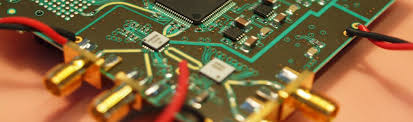
\includegraphics[scale=0.7]{./include/frontimage.png}\\



    % examiners (Referenten)
    \vspace*{1.5cm}
    \LARGE
    \begin{center}
        \begin{tabular}[ht]{l c l}
        \iflanguage{english}{Reviewer}{Referent}: 
            & \hfill & \thesisreviewerone\\
        \iflanguage{english}{Second Reviewer}{Korreferent}: 
            & \hfill & \thesisreviewertwo\\
        % uncomment if you want to provide info on your advisors
        %\iflanguage{english}{Advisor}{Betreuender Mitarbeiter}: 
        %    & \hfill & \thesisadvisorone\\
        %\iflanguage{english}{Second Advisor}{Zweiter betreuender Mitarbeiter}: 
        %    & \hfill & \thesisadvisortwo\\
        \end{tabular}
    \end{center}



    % working time
    \vspace{1cm}
    \begin{center}
        %\large{{Bearbeitungszeit}: 
        \thesistimestart \hspace*{0.25cm} -- %
                                 \hspace*{0.25cm} \thesistimeend
    \end{center}



    % lowest text blocks concerning the KIT
    \begin{textblock}{10}[0,0](2,16.8)
        \tiny{KIT – Die Forschungsuniversität in der Helmholtz-Gemeinschaft}
    \end{textblock}
    \begin{textblock}{10}[0,0](10,16.75)
        \large{\textbf{www.kit.edu}}
    \end{textblock}
\end{titlepage}

    \tikzexternalenable
    \chapter*{Declaration}
I hereby declare that I wrote my master thesis on my own and that I have followed the regulations relating to good scientific practice of the Karlsruhe Institute of Technology (KIT) in its latest form. I did not use any unacknowledged sources or means, and I marked all references I used literally or by content.\\

\vspace{1cm}

\renewcommand{\arraystretch}{0} % for spacing in the tabular environment

\begin{flushright}
	\begin{tabular}{rr}
		Karlsruhe, \thesistimehandin, & \hspace*{5cm}\\[0mm]
		\cline{2-2}\\[2mm]    % the last line has height 2mm due
		& \thesisauthor       % to \arraystretch=0
	\end{tabular}
\end{flushright}

\vfill

\begin{flushright}
	Approved as an exam copy by \\
	\vspace{1cm}
	\begin{tabular}{rr}
		Karlsruhe, \thesistimehandin, & \hspace*{5cm}\\[0mm]
		\cline{2-2}\\[2mm]    % the last line has height 2mm due
		& \thesisreviewerone  % to \arraystretch=0
	\end{tabular}
\end{flushright}

\renewcommand{\arraystretch}{1}

\cleardoublepage

    \chapter*{Abstract}

Analysis of events occurring in the range of femtoseconds is desired in many scientific experiments.
The high temporal resolution needed for measuring such events imposes a great technological challenge for \glspl{daq} and \glspl{adc}.
In order to relax the requirements on the acquisition systems, the so-called optical time-stretch technique is used to stretch the analog input signal in time.
By using this method data converters can be operated at lower sample rate than would be required without it (several \gls{thz} to ). 
Measuring the signal with commercial \glspl{daq}, such as digital storage oscilloscopes, still poses another challenge.
Due to the limited acquisition time windows of such systems, continuous measurements at high sampling rate over a long period of time is not possible.
In applications, where measurements of the long-term evolution of the ultra-fast events with high temporal resolution is necessary, the limited memory size is a large limitation.
Therefore new concepts of \glspl{daq} based on the photonic time-stretch method need to be considered.

In this thesis, a first demonstrator of such a new photonic time-stretch based \gls{daq} system has been developed.
The system consists of a high bandwidth front-end sampling card, mounted on a back-end readout card integrating a new generation of \gls{rfsoc} for readout and processing of the acquired samples. 
%todo photonic time stretch erklären

First, the signal under study is stretched using chirped optical pulses and using the chromatic dispersion in optical fibers.
The signal is measured with a photodetector and sampled by the front-end sampling card.
The front-end sampling card integrates 16 sampling channels, each containing a \gls{tha}. 
The sampling time of these \glspl{tha} can be delayed individually.
In this way the so-called time-interleaving method can be implemented to sample the signal at a higher rate thant that normally possible due to the Nyquist theorem.
The design of the board allows it to be used with the time-stretch method as well as independently from it.
Furthermore, the setup allows for different sampling modes.
In single-channel mode one detector is connected to one sampling channel, therefore allowing to acquire data from up to 16 detectors at the same time with one sampling point per channel.
In the multi-channel mode, several channels are connected to one detector via power-splitter, therefore allowing multiple sampling points for one detector. %todo sample time

The \gls{rfsoc} on the back-end readout card integrates a processing unit and a \gls{fpga}. 
A firmware running on the \gls{fpga} is responsible for programming and controlling the components on the sampling card, as well as collecting the acquired samples and sending it to the following processing system via high-speed connections.
The processing unit, hosting e.g. an operating system or a standalone application, allows for the user to control and monitor the overall system via common periphery, e.g. Ethernet.

The name given to the system is \gls{theresa}.
The high-speed \glspl{adc}, integrated in the read-out card are capable of a sample rate of up to \SI{2.5}{\giga \sample \per \second}.
Using the time-interleaving technique for all available glspl{adc} results in an overall maximal achievable sample rate of \SI{40}{\giga \sample \per \second}.  %todo sample rate of overall system
When used in combination with the time-stretch technique and considering currently achievable time-stretch factors, a time resolution in the range of hundred of femtoseconds is possible. 
\gls{theresa} is therefore suitable to be used in beam diagnostics, e.g. at the \gls{kara}.

\chapter*{Zusammenfassung}
\chapter*{Résumé}
    
	
    \begingroup   % in order to avoid listoffigures and
    \tableofcontents                    % listoftables on new pages
    \listoffigures
    \listoftables
    \endgroup
    \cleardoublepage

	\newacronym{kit}{KIT}{Karlsruhe Institute of Technology}
\newacronym{sr}{SR}{Synchrotron Radiation}
\newacronym{linac}{LINAC}{linear accelerator}
\newacronym{rf}{RF}{Radio Frequency}
\newacronym{ipe}{IPE}{Institute for Data Processing and Electronics}
\newacronym{kara}{KARA}{Karlsruhe Research Accelerator}
\newacronym{kapture}{KAPTURE}{Karlsruhe Pulse Taking Ultra-fast Readout Electronics}
\newacronym{csr}{CSR}{Coherent Synchrotron Radiation}
\newacronym{eo}{EO}{Electro-Optic}
\newacronym{adc}{ADC}{Analog-To-Digital-Converter}
\newacronym{dac}{DAC}{Digital-To-Analog-Converter}
\newacronym{sha}{SHA}{Sample-And-Hold-Amplifier}
\newacronym{tha}{THA}{Track-And-Hold-Amplifier}
\newacronym{pll}{PLL}{Phase-Locked-Loop}
\newacronym{fmc}{FMC}{FPGA Mezzanine Card}
\newacronym{hspce}{HSPCe}{High Serial Pin Count Extension} 
\newacronym{lvcmos}{LVCMOS}{Low voltage complementary metal oxide semiconductor}
\newacronym{lvds}{LVDS}{Low Voltage Differential Signaling}
\newacronym{lvpecl}{LVPECL}{Low-voltage positive emitter-coupled logic}
\newacronym{pcie}{PCIe}{PCI Express}
\newacronym{theresa}{THERESA}{Terahertz Readout Sampling}
\newacronym{rfsoc}{RFSoC}{Radio-Frequency System-On-Chip}
\newacronym{lsb}{LSB}{Least Significant Bit}
\newacronym{dc}{DC}{Direct Current}
\newacronym{ac}{AC}{Alternating Current}
\newacronym{thz}{THz}{tera Hertz}
\newacronym{fwhm}{FWHM}{Full Width At Half Maximum}
\newacronym{fpga}{FPGA}{Field Programmable Gate Array}
\newacronym{lna}{LNA}{Low-Noise-Amplifier}
\newacronym{daq}{DAQ}{Data Acquisition System}
\newacronym{mmic}{MMIC}{Microwave Monolithic Integrated Circuit}
\newacronym{sinad}{SINAD}{Signal-to-Noise-and-Distortion Ratio}
\newacronym{snr}{SNR}{Signal-To-Noise-Ratio}
\newacronym{inl}{INL}{Integral Nonlinearity}
\newacronym{dnl}{DNL}{Differential Nonlinearity}
\newacronym{sfdr}{SFDR}{Spurious-Free Dynamic Range}
\newacronym{rms}{RMS}{Root-Mean-Square}
\newacronym{rss}{RSS}{Root-Sum-Square}
\newacronym{enob}{ENOB}{Effective-Number-Of-Bits}
\newacronym{dbfs}{dBFS}{decibels relative to full scale}
\newacronym{dbc}{dBc}{decibels relative to the carrier}
\newacronym{sjnr}{SJNR}{Signal-to-Jitter-Noise-Ratio}
\newacronym{pcb}{PCB}{Printed Circuit Board}
\newacronym{spi}{SPI}{Serial Peripheral Interface}
\newacronym{vita}{VITA}{VMEbus International Trade Association}
\newacronym{sma}{SMA}{SubMiniature version A}
\newacronym{fs}{FS}{Full-Scale}
\newacronym{ic}{IC}{Integrated Circuit}
\newacronym{emi}{EMI}{Electro-Magnetic Interference}
\newacronym{cml}{CML}{Current Mode Logic}
\newacronym{sdi}{SDI}{Serial Data Interface}
\newacronym{esr}{ESR}{Equivalent-Series-Resistance}
\newacronym{esl}{ESL}{Equivalent-Series-Inductance}
\newacronym{vcxo}{VCXO}{Voltage-Controlled Crystal Oscillator}

    % Contents
    \MainMatter
    \chapter{Introduction}
    		In many scientific applications and experiments the observation of non-repetitive, statistically rare events with very fast occurrences is desired.
As these events might occur on a time range of femtoseconds, real-time measurement systems with fine temporal resolution and capable of long acquisition times are necessary.
This imposes high technological challenges on \glspl{daq} and \glspl{adc}.

One bottleneck in the acquisition of ultra-fast events is the limited performance of commercially available \glspl{adc}. 
The limitation posed by the converters is a trade-off between the dynamic range (\gls{enob}) and sampling rate of the converters.
As the sampling rate increases, ambiguity of the comparators (output neither '0' nor '1') in the \gls{adc} and sampling errors due to clock jitter become major limiting factors on the overall performance. \cite{Mahjoubfar2017}

A first demonstration of a concept to overcome these limitations was presented in 1999 by \cite{ts_adc}. 
The idea is to stretch the analog signal in time before digitizing it in the converter and hence relax the demands on the data converter performance. 
This time-stretching is accomplished by using chirped optical pulses and chromatic dispersion in optical fibers.
The concept is therefore called ``photonic time-stretch'' and was successfully tested in combination with a moderate-speed \gls{adc} in \cite{ts_adc}.

Since then, the time-stretch method has been continuously improved and has found use in many applications.
For example, in biomedical diagnostics, a first demonstration of an artificial intelligence based high-speed phase microscope has been developed. 
It uses \gls{tsqpi}, a technique based on the time-stretch concept which enables simultaneous measurement of phase and spatial intensity profiles.
This allows label-free classification of cells for cancer diagnostics and drug development. \cite{Mahjoubfar2017} 

The time-stretch concept is also useful for applications in particle accelerators due to the short timescales involved.
In a storage ring for example, relativistic electron bunches interact with their own radiation which can lead to the formation of spatial microstructures inside the bunches, a phenomenon also called micro-bunching instability.
This is a source of intense pulses of terahertz radiation (\gls{csr}) and therefore an important field of study. 
A first demonstration of direct observation of these instabilities was performed at the synchrotron facility \gls{soleil} using a time-stretched signal together with a real-time oscilloscope. \cite{Roussel2015}

The use of the time-stretch method in different applications has demonstrated the advantages to measure events with femtosecond resolution.
However, commercially available real-time diagnostics systems are limited in memory space (currently maximal memory depth lies in the range of few Gigasamples). 
This limits the acquisition time of such systems at maximum sampling rate, which lies in the range of a few milliseconds at best.
It is therefore not possible to measure data continuously over a large period of time. 
This creates a problem in applications where a longer observation time (up to hours) is required, e.g. in accelerator applications where the turn-by-turn analysis\footnote{Turn-by-turn denotes the analysis of a specific bunch for every turn, bunch-by-bunch denotes the analysis between individual bunches} of the electron bunches is desired in order to study the evolution of the bunch profiles. 

This challenge was the motivation to design novel ultra-fast acquisition systems based on the photonic time-stretch \gls{adc}. 
Together with the next generation of \gls{fpga}-based systems with integrated high-performance \glspl{adc} this gives rise to a new concept of \gls{daq}, the photonic time-stretch \gls{daq}.
The photonic time-stretch \gls{daq} consists of a photonic part, which consists of the time-stretching section and the conversion of photons into electrical signal with a photo-detector. 
Furthermore, such a system has one or multiple \glspl{adc} converting the analog values into digital signals.
The digital signals are then processed in a computing unit and broadcast to other units as needed if the system is integrated into a cluster of measurement systems. %todo whats the purpose of all this if the system is not integrated? what are other units? more kaptures?
 

\section{Objective}
In this thesis, a first demonstrator of a \gls{daq}-system based on the time-stretch concept is developed.
This system, called \gls{theresa} system, enables high-speed measurements of ultrafast events with a time resolution in the range of femtoseconds.

In order to achieve such high resolution, the time-stretch technique will be used in order to stretch the input signal in the range of pico- to nano-seconds.
The input signal will be continuously sampled by high-speed \glspl{adc} with a temporal resolution defined by the user as needed.
To sample the signal, the \glspl{adc} need to have a sampling rate in the order of several \si{\GHz}.
The amplitudes of the signals to be measured are very small and an appropriate resolution of the \glspl{adc} has to be chosen in order to guarantee an \gls{enob} of at least 10 bits. \cite{bielwaski}

This leads to the next challenge: Sampling at several \si{\GHz} with high resolution, implies a large amount of data, leading to a data rate in the range of Terabits per second.
In order to enable such a high data-throughput, the system will be based on a new generation of \gls{soc}, integrating a \gls{fpga} and a processing unit together with the high-speed \glspl{adc}. 
The \gls{soc} will have high-speed peripherals in order to guarantee the continuous high-speed data-throughput. 
Combination with the \gls{fpga} should allow for flexible system tuning for a user-defined application.
The user will be able to control and configure the system via an application or operating system running on the processing unit.

Furthermore, the system should be compatible with already existing high-speed \gls{daq} frameworks (e.g. based on \gls{pcie}) and be easily integrated into the system for the user application (e.g. through optical fibers to a distributed instrumentation system). 
However, stand-alone operation should also be possible.
Furthermore, the \gls{daq} should be designed in such way that usage independent from the time-stretch method is possible.


%
%The requirements of the \gls{thz} science define the requirements on the newly developed system. 
%It should be able to acquire fast events over a long period of time, allowing to study the evolution of the electron bunch dynamics. 
%Therefore, a high temporal resolution is required, as well as high memory depth and/or high-speed connection in order to send the data to a data processing and storage system. 

The overall thesis is structured in the following way: 
Chapter 2 gives the necessary theoretical background for the new \gls{theresa} system. 
The subject of \gls{thz} science in particular is touched being the main motivation for the design of the novel time-stretch sampling system.
Chapter 3 covers the general architecture of \gls{theresa}, including also state of the art readout-systems, especially the \gls{kapture} which is in operation at the \gls{kara}.
Chapter 4 describes the design steps of the front-end sampling card of \gls{theresa} in detail.
Chapter 5 covers the description of the back-end readout card, as well as the design of the appropriate firmware.
At last, results are concluded and an outlook for the newly developed system is given.
%todo use autoref or ref to have hyperlinks here


\glsresetall

\chapter{Motivation}
As the main aspired use case of the newly developed time-stretch \gls{daq} lies in accelerator physics applications, especially in \gls{thz} science e.g. at \gls{kara}, an introduction into this topic is given in the following section. 

After that the general architecture and basic theory of a photonic time-stretch \gls{daq} is given.
First, the basic working principle of the time-stretch concept is explained.
Then, a short overview of the basic \gls{adc} theory is given, together with the most prominent figures of merit. 
Knowledge and understanding of \gls{adc} characteristics is necessary to evaluate the overall performance of the converter. 

\section{Requirements in THz Science}
Recent years have seen an increasing interest in \gls{thz} radiation, ranging from \SI{3}{\tera \hertz} up to \SI{30}{\tera \hertz}\footnote{At \gls{kara}: \SIrange{0.1}{1.2}{\tera \hertz}}, as it allows non-destructive analysis of organic material. 
This is possible because unlike e.g. X-Rays, \gls{thz} radiation is not ionizing.
It is therefore of great interest to use \gls{thz} radiation in fields like biology, medicine or material science.
However, until recently the usage of \gls{thz} radiation was very limited, as generation of such radiation has proven to be difficult.
%todo what about the usage of thz for spectroscopy since the thz hv-energy matches some interesting bonds in chemistry/bio.

Synchrotrons are a potential source of \gls{thz}-radiation. %todo synchtrons != storage rings (but similar) explained in krieger strahlungsquellen book
The emission of \gls{thz} radiation is closely linked to instabilities of the charged particles which are accelerated in the synchrotron. \cite{mueller2012}
These instabilities occur in the time range of femtoseconds and cause bursts of \gls{thz} radiation.
The periodicity of these bursts depends on multiple parameters of the synchrotron and therefore imposes a challenge on controlling the emission of \gls{thz} radiation.
Studying the dynamics of these instabilities is an important step towards the application of synchrotrons as source of \gls{thz} radiation. \cite{rota2018}



\subsection{Coherent Synchrotron Radiation}
In synchrotron radiation facilities \gls{sr} is produced by accelerating relativistic electrons.
Emission of \gls{sr} occurs, when electron beams are bent or deflected with dipole magnets or using undulators. The latter are used to make the electrons oscillate by generating a periodic magnetic field.  
\autoref{fig:storageRing} shows the general scheme of an electron storage ring.

Electrons, which are grouped to ``electron bunches'', are generated with an electron gun and accelerated to relativistic speeds\footnote{almost speed of light} by a pre-accelerator (often a \gls{linac}, a booster ring accelerator or a microtron with a booster). %todo or microtron + booster
After being brought up to their nominal energy\footnote{in a booster}, the bunches are injected into the storage ring.
In the ring, the path of the electron bunches is altered by dipole magnets, guiding them on a circular trajectory. %todo why in the footnote?
Due to emission of \gls{sr} at each bend, the electrons lose energy, which has to be compensated for.
This is done by accelerating them with an electric field inside a \gls{rf} cavity.
Not shown in the drawing are the beamlines, which lead the \gls{sr} radiation, or rather chosen wavelength ranges, through an optical system to the respective user experiments. \cite{roussel2014,rota2018}

\begin{figure}[tbh]
	\centering
	\includegraphics[width=0.7\textwidth]{chap/02-theory/img/synchrotron.pdf}
	\caption{Basic scheme of an electron storage ring (redrawn from \cite{roussel2014})}
	\label{fig:storageRing}
\end{figure}

The range of \gls{sr} reaches from hard X-rays down to the infrared region of the electromagnetic spectrum (see \autoref{fig:spectrum}). \Gls{sr} shows properties like high intensity, high collimation, polarisation and generation in pulses of well-defined time duration.
High intensity is necessary for better penetration of the matter under study.
It prevents unnecessary exposure of the matter outside the area of interest and  improves the image quality by producing less scatter radiation from these areas.
Well defined duration of the pulses allows to observe chemical reactions on short time scales.
Due to this properties, synchrotrons are used for microscopy, spectroscopy, and time-resolved experiments in such fields like condensed matter physics, biology, material science and many more.

\begin{figure}[H]
	\centering
	\includegraphics[width = \textwidth, height = 0.5\textwidth]{chap/02-theory/img/spectrum.tikz}
	\caption{Electromagnetic spectrum} %todo of what?
	\label{fig:spectrum}
\end{figure}


\paragraph{Karlsruhe Research Accelerator}
At the synchrotron light source \gls{kara}, the possibility to utilize the synchrotron as a source of \gls{thz} is actively researched. 
The photonic time-stretch \gls{daq}, which has been developed in this thesis, should also be integrated into the beam diagnostics system at \gls{kara}. 
Therefore, a short overview of some parameters of this facility has been given below.

\gls{kara} is located at the \gls{kit} and is operated by the \gls{ibpt}.
The storage ring can be filled up with up to 184 electron bunches with a distance of \SI{2}{\nano\second} ($\eqdev$ \SI{500}{\mega\hertz}) between two adjacent bunches.
The main accelerator parameters are listed in \autoref{tab:kara}. 

\begin{table}[tbh]
	\caption{Some KARA parameters \cite{rota2018}}
	\label{tab:kara}
	\centering
	\begin{tabular}{ll}
		\toprule
		\textbf{Parameter}                  & \textbf{Value}                \\ \midrule
		Beam energy (max.)                  & \SI{2.5}{\giga \electronvolt} \\
		Circumference                       & \SI{110}{\meter}              \\
		Revolution Frequency (one electron) & \SI{2.7}{\mega \hertz}        \\
		        \multicolumn{2}{c}{\textbf{Minimum bunch spacing}}          \\
		\quad multi-bunch                   & \SI{2}{\nano \second}         \\
		\quad single-bunch                  & \SI{368}{\nano \second}       \\
		          \multicolumn{2}{c}{\textbf{Bunch length (rms)}}           \\
		\quad normal operation              & \SI{45}{\pico \second}        \\
		\quad short bunch                   & \SI{2}{\pico \second}         \\ \bottomrule
	\end{tabular}
\end{table}

One scientific focus at \gls{kara} lies in the study of so-called ``micro-bunching instabilities'' which are described in the following.

\subsubsection*{Micro-Bunching Instabilities}
Increasing demands in current and future accelerators applications call for higher brilliance of the emitted radiation. 
Brilliance denotes describes both the brightness and the angular spread of the beam. 
Higher brilliance allows to see more detail in the material under study.
The higher brilliance is achieved by shortening the electron bunches. 
As illustrated in \autoref{fig:csr}, this results in emission of \gls{csr}, the spectrum of which spans from \SI{100}{\GHz} up to THz.
Due to this \gls{csr} the bunches interact with their own radiation as shown in \autoref{fig:electronInteract}, which introduces complex longitudinal dynamics.
\begin{figure}[tbh]
	\centering
	\begin{subfigure}{0.4\textwidth}
		\centering
		\includegraphics[height=0.4\textwidth]{chap/02-theory/img/SRincoherent.tikz}  
		\caption{Incoherent SR}
		\label{fig:srincoherent}
	\end{subfigure}
	\hfill
	\begin{subfigure}{0.4\textwidth}
		\centering
		\includegraphics[height=0.4\textwidth]{chap/02-theory/img/SRcoherent.tikz}  
		\caption{Cohenrent SR}
		\label{fig:srcoherent}
	\end{subfigure}
	\begin{center}
		\begin{subfigure}{0.4\textwidth}
			\centering
			\includegraphics[width=1.2\textwidth]{chap/02-theory/img/SRlegend.tikz}  
			\label{fig:srlegend}
		\end{subfigure}
	\end{center}
	\caption[Incoherent and coherent SR]{Incoherent \gls{sr} and coherent \gls{sr} due to shorter electron bunch length \cite{rota2018}}
	\label{fig:csr}
\end{figure}


\begin{figure}[tbh]
	\centering
	\includegraphics[width = 0.8\textwidth]{chap/02-theory/img/electronInteraction.tikz}
	\caption{Electrons interact with their own radiation \cite{Bielawski2019}}
	\label{fig:electronInteract}
\end{figure}
These dynamics are the so called micro-bunching instabilities, the formation of micro-structures (in the sub-millimeter range) in the longitudinal density profile of the electron bunches.
These instabilities occur in bursts and are hard to control, as they depend on a number of system parameters.
This imposes on one side a huge limitation to the stable operation of the overall system at high current density/short bunch length mode.
On the other side, these instabilities themselves emit brilliant \gls{thz} radiation that could be potentially used in imaging applications.
Such applications however require a stable power of the radiation. 
Therefore, a control of these instability bursts could potentially make them a source of \gls{thz} radiation for user-applications. 
A thorough understanding and studying of these beam dynamics is therefore an important step towards providing an applicable \gls{thz} source. \cite{rota2018,brosi}
In order to make such investigations possible, appropriate beam diagnostic systems are required, which are capable of both capturing (ultra-)fast and long-term changes in the bunch profile.  

\subsection*{Control of Micro-Bunching Instabilities}
The \gls{ultrasync} project, funded by ANR-DFG\footnote{\gls{anr}, \gls{dfg}}, has an objective of ultrafast study and control of electron bunches in synchrotron light sources.

There is the question of control (i.e. suppression) of the bursts of \gls{thz} radiation occurring during the micro-bunching instability.
The goal is to obtain a high power and stable coherent emission. 
The current experimental setup uses a relatively simple feedback loop:
\begin{itemize}
	\item A bolometer/Schottky barrier diode detector which produces the input signal for the feedback loop.
	\item A low-cost \gls{fpga} (Red Pitaya) that controls the the accelerating voltage of the synchrotron based on the input
\end{itemize} %todo Red Pitaya?

However, there are limitations in the controllable bunch charge in the accelerator this feedback loop can handle, which is around \SI{10}{\milli \ampere}. 
Therefore, an open question is whether measuring each \gls{thz} pulse using the setup
\begin{itemize}
	\item Electro-Optical sampling and time-stretching
	\item Association with the new \gls{fpga}-based system, i.e. \gls{theresa} system
	\item Finding adequate feedback, programmed in the \gls{fpga}
\end{itemize}
would help in solving the problem and allow the control to succeed also at higher currents (goal: \SI{15}{\milli \ampere}) \cite{bielwaski}.

\subsection{Electro-Optic Techniques for Longitudinal Bunch Profile Diagnostics}
Methods for analyzing the longitudinal profile of electron bunches are based on a similar, if not the same, electro-optical concept as the time-stretch method. 
Two most prominent methods are briefly described for the sake of completeness.
\subsubsection*{Scanning-Type Electro-Optic Sampling}
The scanning-type\gls{eos} samples one point at the time of the \gls{thz} pulse, emitted e.g. from an electron bunch, at each acquisition, hence the naming of this method.

A short laser pulse (duration typically hundreds of femtoseconds) co-propagates with a \gls{thz} pulse from \gls{csr} (range of picoseconds) in an \gls{eo} crystal. 
Due to the Pockels effect the \gls{thz} pulse causes a time dependent birefringence in the crystal.
This modulates the polarization state of the laser pulse.

To sample the pulse, the delay between the laser and the \gls{thz} pulse is varied.
To detect the changing polarization, the polarization of the laser pulse is transformed into an intensity modulation. This is done by using polarizers, e.g. \glspl{qwp} and \gls{wp} (as shown in \autoref{fig:scan_eo}).
A general scheme of the system is shown in \autoref{fig:scan_eo}.
For this technique a stable emission of the \gls{thz} pulses is crucial, as they are not measured in one acquisition. \cite{roussel2014}
\begin{figure}[tbh]
	\centering
	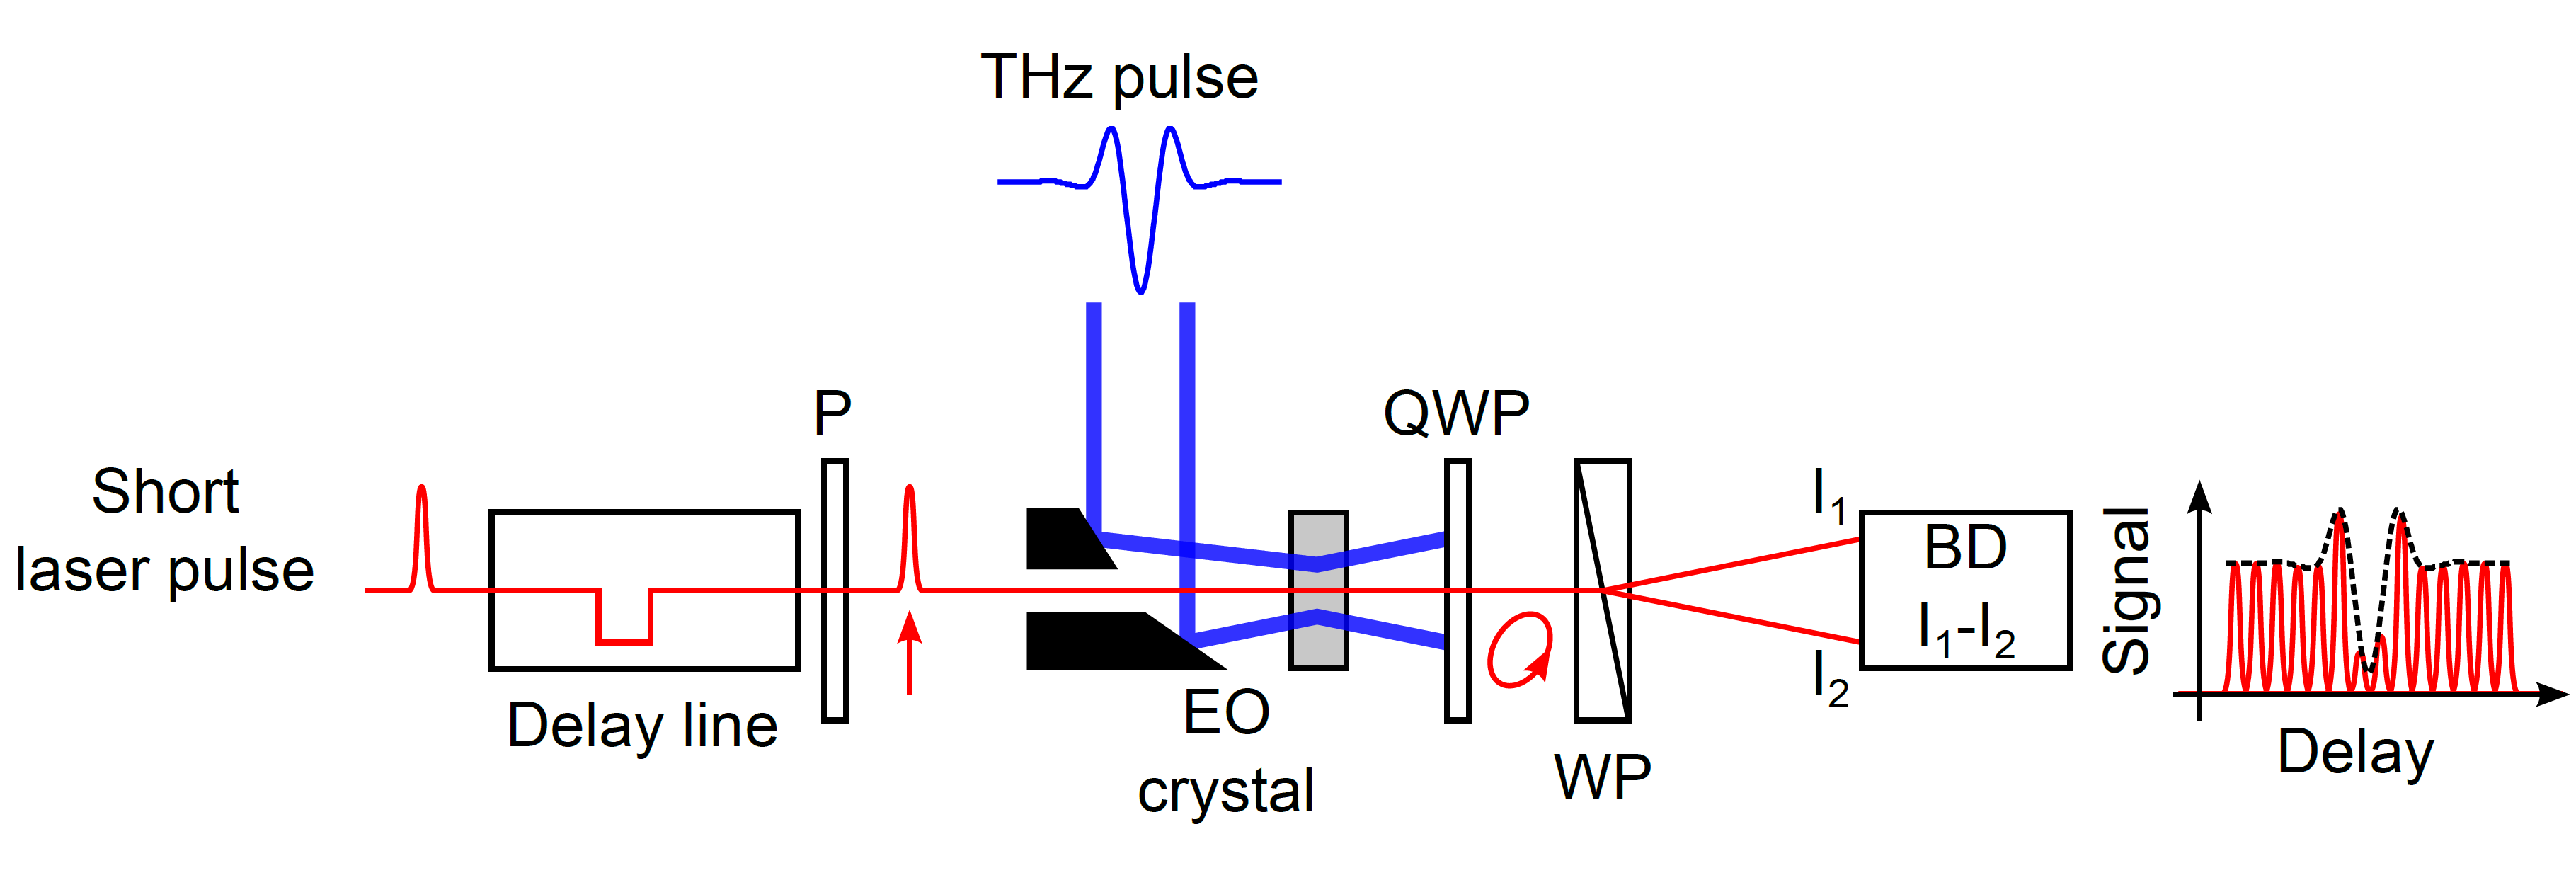
\includegraphics[width = \textwidth]{chap/02-theory/img/scanning_eo}
	\caption{Scheme of Scanning-Type Electro-Optical Sampling System \cite{roussel2014}}
	\label{fig:scan_eo}
\end{figure}


\subsubsection*{Spectrally Resolved Electro-Optic Detection}
In contrast to the \gls{eos}, single-acquisition is possible with the spectrally resolved \gls{eo} detection technique.
The short laser pulse is first stretched to a duration similar to the \gls{thz} pulse in a dispersive material, called stretcher.
In this way the pulse is chirped, meaning the instantaneous frequency of the pulse varies over time.
Together with the \gls{thz} pulse, the laser pulse propagates through an \gls{eo} crystal.
Again, the induced birefringence modulates the laser pulse, not only in time, but also in the spectral domain. %todo 'not only' -> due to the time/spectral duality or sth
The polarization state of the pulse is converted into an amplitude/intensity modulation.
This is done with a series of \gls{qwp}, \gls{hwp} and a polarizer (P) (as shown in \autoref{fig:spectral_eo}).
To retrieve the \gls{thz} pulse shape in time, the spectrum of the laser pulse is measured with a spectrometer. %todo what spectrometer (optical or electrical) or state model
A general scheme of the system is shown in \autoref{fig:spectral_eo}. \cite{roussel2014}

\begin{figure}[tbh]
	\centering
	\includegraphics[width = \textwidth]{chap/02-theory/img/spectral_eo}
	\caption{Scheme of Spectrally Encoded Electro-Optical Detection System \cite{roussel2014}}
	\label{fig:spectral_eo}
\end{figure}

The temporal resolution of this method is limited due to the finite chirp rate
\begin{equation}
	\text{chirp rate} = \frac{\text{laser bandwidth}}{\text{laser pulse duration after stretcher}}.
\end{equation}

The minimal resolution $T_{\text{min}}$ depends on the bandwidth-limited pulse duration (before stretcher) $T_0$ and the duration of the chirped laser pulse $T_c$:
\begin{equation}
	T_{\text{min}} = \sqrt{T_0 T_c}
\end{equation}


\section{Photonic Time-Stretch Method}
The operating principle of the optical time-stretch technique can be described in three steps (see \autoref{fig:eo_ts}).

First, a short laser pulse (duration typically hundreds of femtoseconds) propagates in a dispersive medium, e.g. an optical fiber of length $L_1$ (see \autoref{fig:eo_ts}).
With the optical bandwidth of the laser pulse $\Delta \lambda$ and the dispersion parameter $D_1$ of the fiber, this results in a chirped laser pulse of the duration
\begin{equation}
	T_1 = \Delta \lambda D_1 L_1.
\end{equation}
The next step is the time-to-wavelength-mapping, where a temporal intensity modulation is imprinted on the chirped pulse.
This happens when the laser pulse co-propagates with another pulse, e.g. a \gls{thz} pulse from \gls{csr} (duration in the range of picoseconds), in an \gls{eo} crystal. 
Due to the Pockels effect the \gls{thz} pulse causes a time-dependent birefringence in the crystal. 
The Pockels effect describes the phenomenon of occurring and change of existing birefringence in an electric field, which is linearly proportional to the electric field strength. \cite{pockels} 

After that, the modulated chirped pulse propagates through another dispersive medium, a fiber of the length $L_2$.
In this way, the temporal modulation of the pulse is further stretched to the duration $T_2$, which is long enough for detection with photodetectors and the digitizing with \Glspl{adc}. \cite{roussel2014} 

The factor $M$, by which the pulse is slowed down, is calculated as
\begin{equation}\label{eq:ts}
	M = 1 + \frac{L_2}{L_1}.
\end{equation}
As example, assume the length of the dispersive media as $L_1 = \SI{10}{\meter}$ and $L_2 = \SI{2}{\kilo \meter}$ and an input signal with the duration $t_\text{sig} = T_1 = \SI{1}{\pico \second}$. 
With \autoref{eq:ts} the stretching factor for this set-up is $M \approx 200$. The input pulse is stretched to $T_2 = M \cdot T_1 = 200 \cdot \SI{1}{\pico \second} = \SI{200}{\pico \second} = \SI{0.2}{\nano \second}$.
This corresponds to a frequency of $\SI{5}{\GHz}$ which is much easier to handle e.g. for an oscilloscope.

\begin{figure}[tbh]
	\centering
	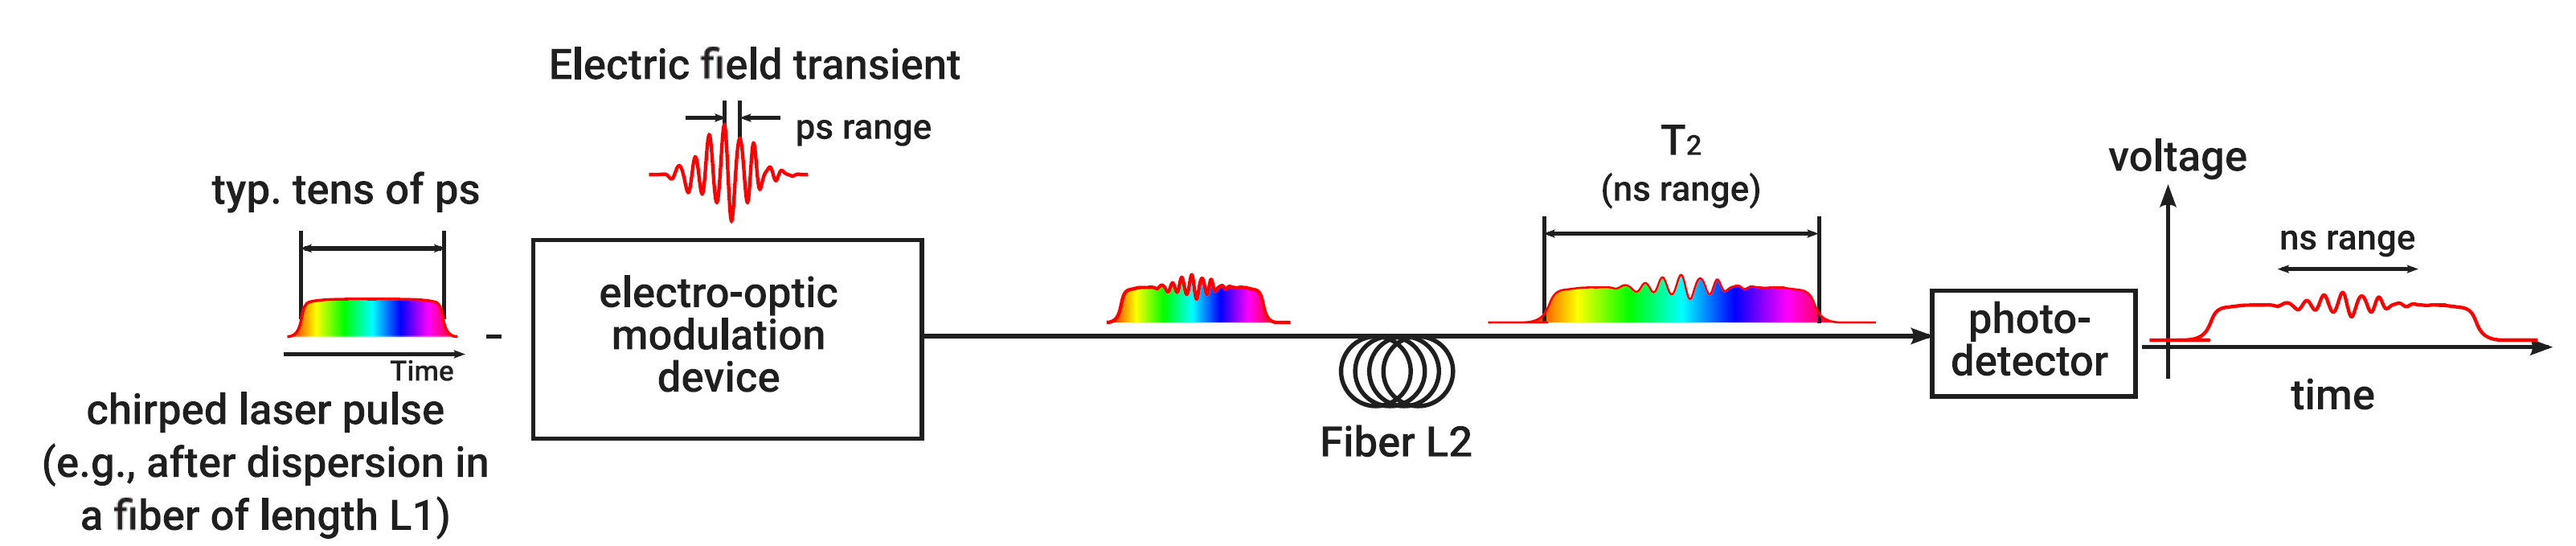
\includegraphics[width = \textwidth]{chap/02-theory/img/time_stretch.png}
	\caption{Working principle of the electro-optical time-stretch technique \cite{roussel2014}}
	\label{fig:eo_ts}
\end{figure}

\paragraph{Photodetector}
In order to convert the time-stretched optical signal into an electrical value a photodetector, e.g. a photodiode, is needed.
A basic diode photodetector is a photo-diode operated in reverse bias, meaning the $p$-side is connected to the negative terminal and the $n$-side to the positive terminal of the power supply. %todo typically with some resistor to set the op and not fry the diode
This enlarges the depletion region (see \autoref{fig:pn_junc}) of the $p/n$-junction as the depletion region contains only a very small amount of free charge carriers. 
Irradiating diode with photons of sufficient energy generates electron-hole pairs due to the photoelectric effect. %todo check my changes
If the electron-hole pairs are produced in the depleted region of the $p/n$-junction, they are separated by the electric field applied across it, before they can recombine. 
This creates a so called photo-current which can be measured. \cite{photodiode} %todo with a trans impedance amplifier maybe for the 'voltages' in the next section

\begin{figure}[tbh]
	\centering
	\includegraphics[]{chap/02-theory/img/pn.tikz}
	\caption{pn-junction with depleted region \cite{pn-junc}}
	\label{fig:pn_junc}
\end{figure}


\section{Analog-To-Digital Converter}
\Glspl{adc} are used to translate analog signals, like voltages, into the digital representation of these signals.
This \textit{digitized} version can then be stored and processed by information processing, computing, data transmission and control systems. 
This translation, also called ``conversion'', can be seen as encoding a continuous-time analog input $V_\text{in}$ (voltage) into a series of discrete, $N$-bit words. %todo $V_\text{in}(t)$ ?
This process is also called \textit{sampling}. 
With the full-scale voltage of the $V_{\text{FS}}$, the individual output bits $b_k$ and the quantization error $\epsilon$, the \gls{adc} should satisfy the relation
\begin{equation} \label{eq:adc_sample}
	V_{\text{in}} = V_{\text{FS}} \sum_{k = 0}^{N-1} \frac{b_k}{2^{k+1}} + \epsilon.
\end{equation}
%todo what is full scale voltage, lsb, v_q, \epsi?
This can also be rewritten in terms of the \gls{lsb} or quantum level $V_Q$
\begin{equation}
	1 \text{LSB} = \frac{V_\text{FS}}{2^N} = V_Q.
\end{equation}
With \autoref{eq:adc_sample} this leads to 
\begin{equation}
	V_\text{in} = V_Q \sum_{k = 0}^{N-1} b_k 2^{k}  + \epsilon.
\end{equation}

\autoref{fig:idealADC} shows the ideal transfer function of a 3-bit \gls{adc}. 
Each digital $N$-bit word corresponds to a range of input voltage values (\textit{code width}), which is centered around a \textit{code center}.
The input voltage is resolved to the code of the nearest code center.
\begin{figure}[H]
	\centering
	\includegraphics[width = 0.7\textwidth]{chap/02-theory/img/ideal_adc}
	\caption[Transfer function of ideal, 3-bit ADC]{Transfer function of an ideal, 3-bit \gls{adc} (redrawn from \cite{Lundberg})}
	\label{fig:idealADC}
\end{figure}


\paragraph{Sample-And-Hold-Amplifier}
\Glspl{adc} need a certain amount of time to sample the input signal.
If the level of the analog signal changes by more than one \gls{lsb} during this period, this can result in large errors in the output signal.
Therefore so called \gls{sha} are used in front of the \gls{adc} to hold the input level constant for the needed amount of time.

A general block diagram of a \gls{sha} is shown in \autoref{fig:tha}. %todo correct figure? THA vs SHA?
It consists of an input and output buffer, a switch controlled by the sampling clock and a capacitor.
The analog input is buffered in an input buffer which leads to a switch that is controlled by a sampling clock.
During the sample mode, i.e. during the negative sampling clock cycle, the switch is open.
At the transition from negative to positive clock cycle, the switch closes, connecting the input signal with the capacitor which is charged in this way.

The \gls{adc} sampling time needs to be timed in such way, that the whole duration of an analog-to-digital conversion falls into the hold period of the \gls{sha} and does not exceed into the sample period. 
\autoref{fig:sha_timing} shows a qualitative example for proper sample timing. 
As conclusion, the upper frequency limitation is not determined by the \gls{adc} itself, but rather by the aperture jitter, bandwidth, distortion, etc. of the \gls{sha}. \cite{walt}

\begin{figure} [H]
	\centering
	\tikzexternaldisable
	\includegraphics[width=\linewidth]{chap/02-theory/img/sha_timing.tikz}  
	\tikzexternalenable
	\caption[SHA timing example]{Example for appropriate sampling timing when using Sample-And-Hold-Amplifier. The sample points of the \gls{adc} should be inside the period, where the \gls{sha} holds the input value.}
	\label{fig:sha_timing}
\end{figure}
\paragraph{Track-And-Hold Amplifier}
Apart from the \glspl{sha} there also exists the so called \gls{tha}.
Though the names are often used interchangeably, there exists one fundamental difference between a \gls{sha} and a \gls{tha}.
Strictly speaking, the output of a \gls{sha} is not defined during the sample period. 
Only when switching to the hold mode, the output is assigned to a defined value: the voltage level at the input in that moment.
Contrary to that, the \gls{tha} acts as a unity gain amplifier during the sample period, meaning the output is just a replication of the input. 
The \gls{tha} ``tracks'' the input signal (see also \autoref{fig:sha_timing}).
Therefore, instead of speaking of a ``sample'' period, the term used here is the ``track'' period.
When switching to hold mode, the instantaneous input level is held over the course of the hold period.
This principle allows to improve the sampling rate, as the settling time of an \gls{tha} is in general smaller than one of a \gls{sha}.
Settling time denotes the amount of time needed for the output voltage to be at a stable level, after the transition from track/sample to hold mode.
This process is quicker, when the output voltage is already in the range of the sampled input at the moment, instead of when the hold capacitor first has to be charged to the input voltage. \cite{Reeder2017}


\begin{figure}[tbh]
	\centering
	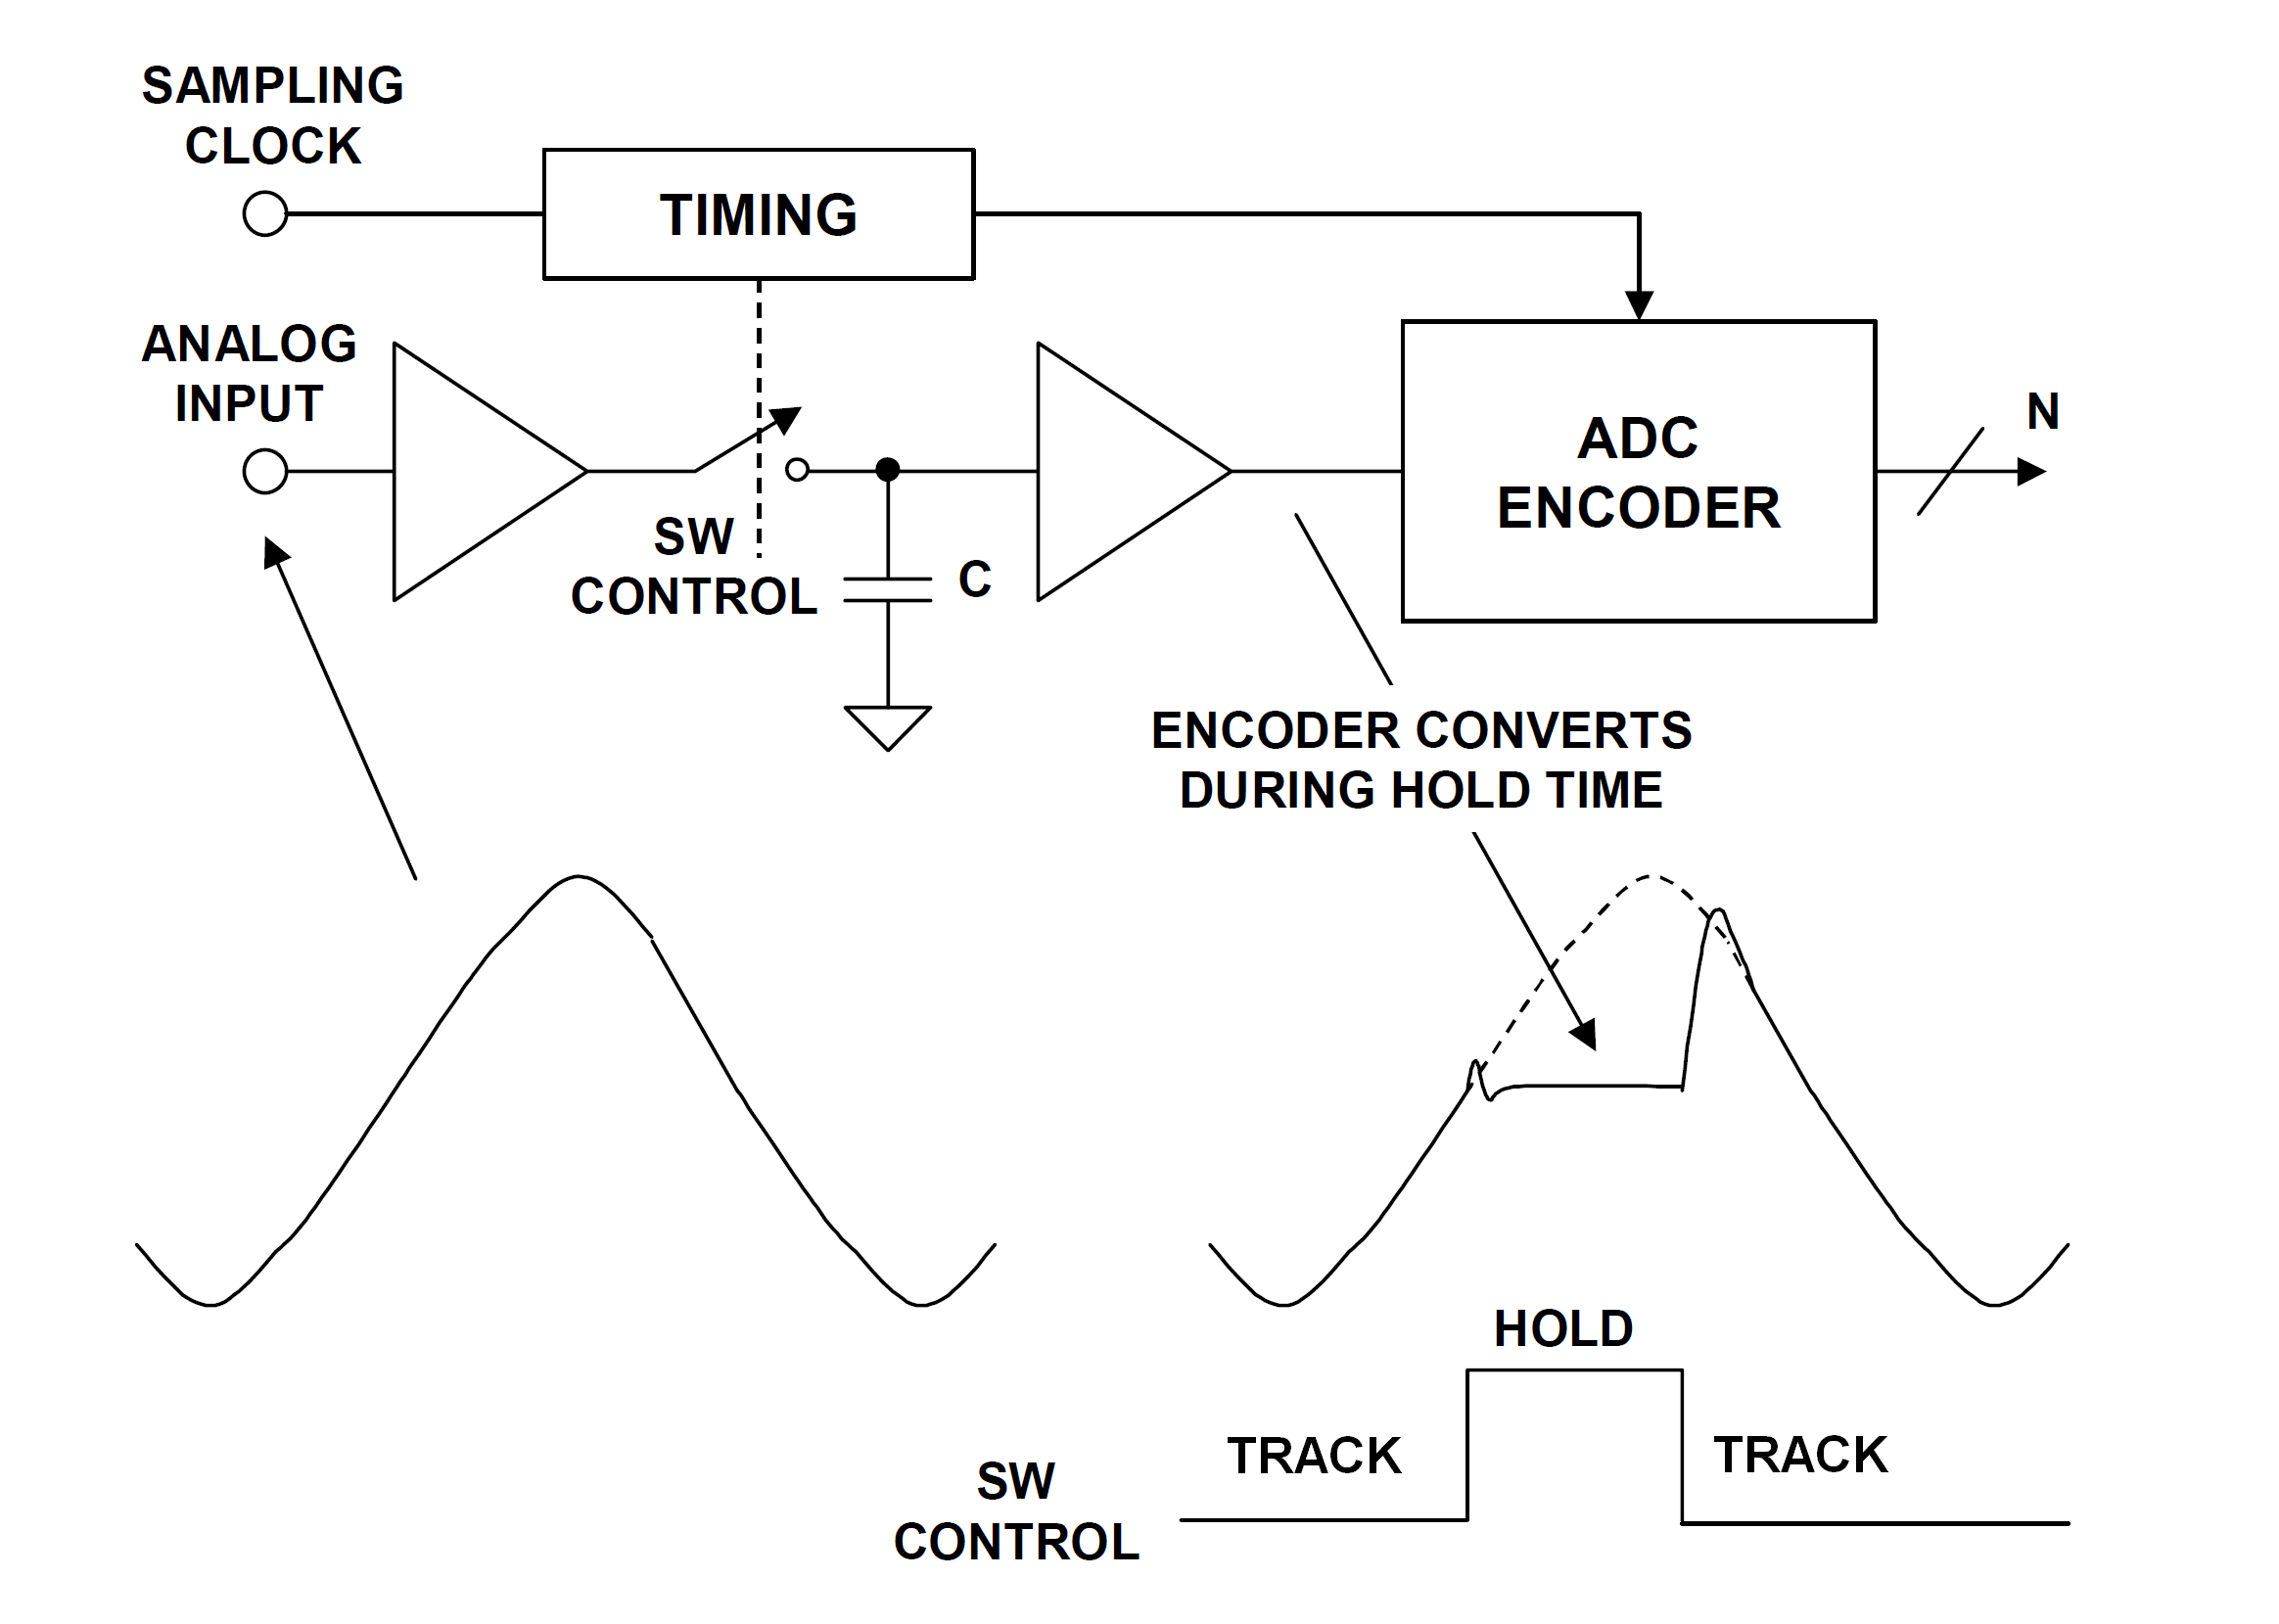
\includegraphics[width = \textwidth]{chap/02-theory/img/tha}
	\caption{Track-And-Hold-Amplifier schematic and principle \cite{walt}}
	\label{fig:tha}
\end{figure}

\subsection{Characteristics of Analog-To-Digital-Converters}\label{ssec:adc_charac}
For an ideal converter, the number of bits and the sampling rate would be sufficient to fully characterize its performance.
Real \glspl{adc} however differ from the ideal behavior by introducing static and dynamic imperfections.
Different applications have different requirements, which leads to a number of specifications.
These can be divided into the categories according to \cite{Lundberg}:
\begin{itemize}[noitemsep]
	\item Quantization Noise
	\item Static parameters
	\item Frequency-domain dynamic parameters
	\item Time-domain dynamic parameters
\end{itemize} %todo which of those are static, which dynamic?
This section provides an overview of these figures of merit.
Which of them are needed to specify the necessary performance of the \gls{adc} has to be chosen for each application accordingly.

\subsubsection{Quantization Noise}\label{par:quant_noise}
Even an ideal $N$-bit converter has errors resulting from the quantization process which behave like noise. %todo maybe can be modelled as noise, or shows as noise instead of behave
The reason is that each $N$-bit word represents a certain range of analog input values, which is 1 \gls{lsb} wide and centered around a code center (see \autoref{fig:idealADC}). \cite{Lundberg}
The input voltage is assigned to the word of the nearest code center.
This means that there will always be a difference between the corresponding voltage of the respective digital code $x_q(t)$ and the actual analog input voltage $x(t)$.
This difference is called the \textit{quantization error}. For an equidistant quantization, the quantization error for a code width $q$ is (see \cite{puente2015})
\begin{equation}
	\left| e_q(t) \right| = \left| x(t) - x_q(t) \right| \leq \frac{q}{2}.
\end{equation}
A setup in order to measure this quantization error is shown in \autoref{fig:qe_m}. 
\begin{figure}[tbh]
	\centering
	\includegraphics[width = \textwidth]{chap/02-theory/img/quant_err_meas.tikz}
	\caption[Measurement setup for quantization error]{Setup for measuring the quantization error of an (ideal) \gls{adc} with input signal $x(t)$}
	\label{fig:qe_m}
\end{figure}

The output of the \gls{adc}, the $N$-bit code corresponding to the voltage level of the input signal $x(t)$, is fed to a \gls{dac}, which converts this code into a corresponding voltage level $x_q(t)$. 
The difference between $x(t)$ and $x_q(t)$ is the quantization error $e_q(t)$.

In order to analyze the quantization noise and the resulting theoretical (maximum) \gls{snr} of the ideal \gls{adc}, assume a ramp with the slope $s$ as an input signal. 
Then, the quantization error $e_q(t)$ can be approximated with a sawtooth signal in the time domain (see \cite{walt}): 
\begin{equation}\label{eq:qe_saw}
	e_q(t) = st, \quad -\frac{q}{2s} < t < \frac{q}{2s} 
\end{equation}
The function in \autoref{eq:qe_saw} is plotted in \autoref{fig:eq}.
\begin{figure}[tbh]
	\centering
	\includegraphics[width = 0.7\textwidth]{chap/02-theory/img/quantization_error.tikz}
	\caption{Quantization noise as function of time (redrawn from \cite{walt})}
	\label{fig:eq}
\end{figure}

The power of this quantization noise can be calculated as the mean-square $e_{\text{rms}}^2$ of $e(t)$ (see \cite{walt}):
\begin{equation}
	P_{QN} = e_{\text{rms}}^{2} = \overline{e^{2}(t)} = \frac{s}{q}\int_{-q/2s}^{+q/2s} (st)^{2} dt = \frac{s^3}{q} \left[ \frac{t^3}{3}\right]_{-\frac{q}{2s}}^{+\frac{q}{2s}} = \frac{q^2}{12}
\end{equation}

In order to calculate the maximal \gls{snr} of an ideal converter, a full-scale input sine wave is applied to the input:
\begin{equation}
	u(t) = u_s \sin(2\pi f t) = \frac{2^{N}q}{2}\sin(2\pi f t)  = 2^{N-1}q \sin(2\pi f t)
\end{equation}
With the effective value of the signal amplitude
\begin{equation}
	u_{\text{eff}} = \frac{u_s}{\sqrt{2}} = \frac{2^{N-1}q}{\sqrt{2}}
\end{equation}
the \gls{snr} can be calculated as 
\begin{equation}
	\text{SNR} = \frac{P_{\text{signal}}}{P_{\text{noise}}} = \frac{u_{\text{eff}}^{2}}{e_{\text{rms}}^{2}} = \frac{2^{2N-2}q^2/2}{q^2/12} = 2^{2N} \cdot 1.5.
\end{equation}
In decibel, the \gls{snr} is calculated as (see \cite{puente2015, walt}):
\begin{equation}\label{eq:idealSNR}
	\text{SNR}|_{\text{dB}} = 10\log\left(2^{2N}\cdot 1.5\right) = 6.02 N + 1.76
\end{equation}




\subsubsection{Static parameters}
\textit{Static parameters} are specifications, which can be measured at low speed/DC. 
\paragraph{Accuracy}
\textit{Accuracy} is the total error with which an \gls{adc} can convert a known voltage, which includes the effects of (see \cite{Lundberg}):
\begin{itemize}[noitemsep]
	\item Quantization error
	\item Gain error
	\item Offset error
	\item Non-linearities
\end{itemize}

\paragraph{Resolution}
\textit{Resolution} is the number of bits $N$ of the \gls{adc}.
Depending from the resolution are the size of the \gls{lsb}, which in its turn determines the dynamic range, code widths and quantization error.
\paragraph{Dynamic Range}
The \textit{dynamic range} represents the ratio between smallest possible output (\gls{lsb} voltage) and the largest possible output (full-scale voltage).
It can be calculated as
\begin{equation}
	20 \log 2^{N} \approx 6N.
\end{equation}

\paragraph{Offset and Gain Error}
The \textit{offset error} is defined as the deviation of the actual \gls{adc} transfer function from the ideal \gls{adc} transfer function in the point of zero. It is measured in \gls{lsb}. 
 
\textit{Gain Error} defines the deviation of the slope of the line going through the zero and full-scale point of the transfer function. %todo state eq for 'transfer function' otherwise 'line', 'zero' and 'full-scale point' undefined here
\autoref{fig:offsetErr} visualizes the effects of both offset and gain error. 
\begin{figure}[tbh]
	\centering
	\includegraphics[width = 0.8\textwidth]{chap/02-theory/img/adc_offset_gain.tikz}
	\caption[Effects of Offset and Fain error in ADC]{Offset and Gain Error in the \gls{adc} characteristic transfer function. The offset error is indicated with the red arrow. The gain error expresses itself via different slope of the real \gls{adc} (dotted) compared to the ideal \gls{adc} (dashed)}
	\label{fig:offsetErr}
\end{figure}

These errors can easily be corrected by calibration. 
In order to measure the offset and gain error, two different voltage levels $V_1$ and $V_2$ are applied at the \gls{adc} input. 
This results in corresponding bit codes $b_1$ and $b_2$.
The slope $s$ of the transfer function can then be calculated by
\begin{equation}
	s = \frac{b_2 - b_1}{V_2 - V_1}.
\end{equation}
From this, the gain error can be determined.
In order to obtain the offset error $b$, the linear equation
\begin{equation}
	b = b_1 - s\cdot V_1
\end{equation}
is solved.


%todo where is this full-scale point here in the fig?

\paragraph{Integral and Differential Non-Linearity Distortion} 
\gls{inl} is the distance of the code centers on the actual \gls{adc} transfer function from the ideal line (dashed line in \autoref{fig:nld}). %todo which transfer function?
It results from the integral non-linearities of the front-end, \gls{sha} and also the \gls{adc} itself \cite{walt, Lundberg}. 

\gls{dnl} is the deviation in actual code width from the ideal width of 1 \gls{lsb}. This non-linearity stems exclusively from the encoding process in the \gls{adc} \cite{Lundberg,walt} . 

The effect of these errors is shown in \autoref{fig:nld}.
\begin{figure}[tbh]
	\centering
	\includegraphics[width = 0.8\textwidth]{chap/02-theory/img/nonlinear.tikz}
	\caption[ADC Nonlinearities]{Transfer function of a real \gls{adc} showing \gls{dnl} and \gls{inl}.\cite{Lundberg}}
	\label{fig:nld}
\end{figure}

These non-linearities could be measured with a histogram test.
A voltage ramp is applied at the input and the number of occurrences of each \gls{adc} output code, $n$(code), is measured.
With the ramp slope $s$ am ideal \gls{adc} with the sampling frequency $f_s$ would give
\begin{equation}
	n(\text{code}) = \frac{\text{LSB}}{s} \cdot f_s = n_\text{avg},
\end{equation}
which ideally would be constant for the whole input range (except for the first and last code).
For a real \gls{adc} this is not the case and the \gls{dnl} and \gls{inl} are calculated as (see \cite{inlDnl})
\begin{align}
	\text{DNL(code)} &= \frac{n(\text{code})-n_\text{avg}}{n_\text{avg}}\\
	\text{INL(code)} &= \sum_{i = 0}^{\text{code}} \text{DNL}(i).
\end{align}


\subsubsection{Frequency-Domain Dynamic Parameters}
Any real \gls{adc} is subject to noise distortion. 
\textit{Noise} denotes any unwanted random signal, which interferes with the measuring of the desired signal. 
Examples are quantization noise or random fluctuations due to thermal noise. 
\textit{Distortion} is the term for alteration of the shape of the original signal. 
As an example, distortion of the amplitude might result due to not equal amplification of the parts of a signal. \cite{nd}

In an \gls{adc} (with built-in \gls{sha}) there are a couple of sources, which introduce noise and distortion:
\begin{itemize}
	\item \textbf{Input Stage:} Wideband noise, non-linearity and bandwidth limitation
	\item \textbf{\gls{sha}:} Non-linearity, aperture jitter(see paragraph about Time-Domain Dynamic Performances) and bandwidth limitation %todo use label/autoref here
	\item \textbf{\gls{adc}:} Quantization noise, non-linearity
\end{itemize}

For quantification of noise and distortion, frequency-domain metrics are used. 
Therefore the figures of merit described in the following paragraphs are also called frequency-domain dynamic parameters. 
These parameters are measured with the help of the \gls{fft} meaning any modern oscilloscope can be used to quickly assess the frequency-domain dynamic performance for a given input at the \gls{adc}.
As some parameters, such as \gls{sfdr}, are only defined for one carrier input frequency, several measurements at different input frequencies need to be made in order to fully characterize the \gls{adc}.

In the following paragraphs, an overview of the metrics for quantification of the noise and distortion of an \gls{adc} is given. 


\paragraph{Signal-to-Noise Ratio}
The \gls{snr} is defined as the ratio of the input signal power to the power of the noise signal. 
It is expressed in dB and can be calculated using the \gls{rms} value of the signal and noise amplitudes (see \cite{xilinx_adc}):
\begin{align}
	\text{SNR} &= \frac{\text{Power}_\text{Signal}}{\text{Power}_\text{Noise}}\\
	&= \left( \frac{\text{Amplitude}_\text{Signal,rms}}{\text{Amplitude}_\text{Noise,rms}} \right)^2\\
	&= 20 \log \left( \frac{V_\text{in,rms}}{V_\text{Q,rms}}\right) 
\end{align}
Usually, the \gls{snr} degrades at higher frequencies due to sampling jitter. \cite{xilinx_adc}

\paragraph{Signal-to-Noise-and-Distortion Ratio}
\gls{sinad} (also called SNDR or S/N+D) denotes the ratio between the \gls{rms} of the signal amplitude to the mean value of the Root-Sum-Square (RSS) of all other spectral components, including harmonics, but excluding \gls{dc} (\SI{0}{\hertz}). 
\gls{sinad} is a good indication over the general dynamic performance of the \gls{adc}, as it includes all contributions from noise and distortion.
The higher the \gls{sinad} the stronger the input power is differentiated from noise and spurious components. 

\gls{sinad} can be calculated from the average power of the input signal $P_\text{signal}$, noise $P_\text{noise}$ and $P_\text{distortion}$:
\begin{equation}
	\text{SINAD} = 10 \log \left( \frac{P_\text{signal}}{P_\text{noise} + P_\text{Distortion}} \right)
\end{equation}
It is commonly expressed in dB, \gls{dbc} or \gls{dbfs}.

\paragraph{Effective-Number-Of-Bits}
The \gls{enob} expresses the \gls{sinad} in terms of bits. It can be calculated as (see \cite{walt2009})
\begin{equation}
	\text{ENOB} = \frac{\text{SINAD}-\SI{1.76}{\decibel}}{\SI{6.02}{\decibel}/\text{bit}}. \quad 
\end{equation}
This is derived from solving the equation of the ``ideal \gls{snr}'' (\autoref{eq:idealSNR}) for the number of bits $N$ and substituting \gls{snr} with \gls{sinad}.
This however means, that this parameter assumes a full-scale input signal. Expressing the \gls{enob} for a smaller signal amplitude requires measuring the \gls{sinad} at this level and a correction factor. \cite{walt}

\paragraph{Spurious-Free Dynamic Range}
\gls{sfdr} indicates the dynamic range of the converter, which can be used, before there is interference or distortion from spurious components with the fundamental signal. \cite{Lundberg} 
The \gls{sfdr} is calculated as the \gls{rms} value of the fundamental signal to the \gls{rms} value of the worst spurious signal, i.e. the highest spur in the spectrum.
It is measured over the whole Nyquist bandwidth from \gls{dc} to $f_s/2$, with $f_s$ being the \gls{adc} sampling rate. The spur may or may not be a harmonic of the fundamental signal. \cite{walt2009, Lundberg}

The \gls{sfdr} is an important characteristic in the sense, that it indicates the smallest signal which can still be distinguished from a strong interfering signal. \cite{walt2009} 

The \gls{sfdr} in dBc can be calculated as (see \cite{xilinx_adc})%todo what is dbc?
\begin{equation}
	\text{SFDR}_\text{dBc} = 20 \log \left( \frac{\text{Fundamental Amplitude (RMS)}}{\text{Largest Spur Amplitude (RMS)}} \right).
\end{equation}


\autoref{fig:sfdr} illustrates the \gls{sfdr} in terms of \gls{dbfs} and \gls{dbc}.

\begin{figure}[tbh]
	\centering
	\includegraphics[width = \textwidth]{chap/02-theory/img/sfdr.tikz}
	\caption[SFDR definition]{Visualization of the \gls{sfdr}. It can be indicated either with reference to the carrier frequency in ``dBc'' or with reference to the Full-Scale Input in ``dBFS''. \cite{walt2009}}
	\label{fig:sfdr}
\end{figure}
\paragraph{Total Harmonic Distortion}
The \textit{Total Harmonic Distortion} describes the ratio of the \gls{rms} sum of the first five harmonic components (or aliased versions of them) to the \gls{rms} of the considered fundamental signal. \cite{Lundberg}

\paragraph{Effective Resolution Bandwidth}
\textit{Effective Resolution Bandwidth} denotes the frequency of the input signal, at which the \gls{sinad} has fallen by \SI{3}{\decibel} ($\eqdev$ 0.5 bit in terms of \gls{enob}) compared to the \gls{sinad} at lower frequency range. \cite{Lundberg}

\paragraph{Analog Input Bandwidth}
\textit{Analog Input Bandwidth} is the analog input frequency at which the power of the fundamental is reduced by 3dB with respect to the low-frequency value. \cite{Lundberg}
It is not to be confused with the maximal analog input frequency which the \gls{adc} is able to sample.

\paragraph{Full-Linear Bandwidth}
The \textit{Full-Linear Bandwidth} is defined as the frequency at which the slew-rate of the \gls{sha} starts to distort the input signal by a specified value. \cite{Lundberg} 
The slew-rate (SR) is defined as the rate of how much the voltage $v$ changes over time $t$:
\begin{equation}
	\text{SR} = \frac{\text{d}v}{\text{d}t}
\end{equation}
A slew-rate of \SI{1}{\volt \per \micro \second} for example means, that the output of the amplifier can not change more than \SI{1}{\volt} over the course of \SI{1}{\micro \second}.\cite{2021Slew} 

\paragraph{Time-Domain Dynamic Parameters}
Time-Domain Dynamic parameters describe the deviation of the converter's behavior from the ideal one in time domain. 

\paragraph{Aperture Delay}
\textit{Aperture Delay} (or \textit{aperture time}) is defined as delay between the triggering of the converter (e.g. rising edge of the sampling clock) and the actual conversion of the input voltage into the digitized value. \cite{Lundberg}

\paragraph{Aperture Jitter}
\textit{Aperture jitter} describes the sample-to-sample variation in aperture delay. Jitter can cause significant error in the voltage and decreases the overall \gls{snr} of a converter.
Especially for high-speed \glspl{adc} jitter poses a limit in performance.

Assuming a full-scale sinus-wave $V_{\text{in}}$ as input signal with 
\begin{equation}
	V_{\text{in}} = V_{\text{FS}} \sin(\omega t)
\end{equation}
the maximal slope of this signal is then
\begin{equation}
	\frac{\text{d}V_{\text{in}}}{\text{d}t}\Bigr|_{\text{max}} = \omega V_{\text{FS}}
\end{equation}
Aperture jitter $\Delta t_{\text{rms}}$ occurring during the sampling of this maximal slope produces the \gls{rms} voltage error 
\begin{equation}
	\Delta V_{\text{rms}} = \omega  V_{\text{FS}} \Delta t_{\text{rms}} = 2 \pi f  V_{\text{FS}} \Delta t_{\text{rms}}.
\end{equation}
As variations in aperture time occur randomly, these errors behave like a random noise source. This way, a \gls{sjnr} can be defined as
\begin{equation}
	\text{SJNR} = 20 \log \left( \frac{V_{\text{FS}}}{\Delta V_{\text{rms}}} \right) = 20 \log \left( \frac{1}{2 \pi f  V_{\text{FS}}} \right)
\end{equation}

The voltage error due to jitter and the \gls{sjnr} for different aperture jitter values are shown in \autoref{fig:ap_jit}.

\begin{figure}[tbh]
	\centering
	\begin{subfigure}{0.48\textwidth}
		\centering
		\includegraphics[width=\textwidth]{chap/02-theory/img/jitterTimeDomain.tikz}  
		\caption{Effect of aperture jitter}
		\label{fig:jitter}
	\end{subfigure}
	\hfill
	\begin{subfigure}{0.48\textwidth}
		\centering
		\includegraphics[height=\textwidth]{chap/02-theory/img/SJNRjitter.tikz}  
		\caption{SJNR for different aperture jitter values}
		\label{fig:sjnr}
	\end{subfigure}
	\caption[Aperture jitter and SJNR]{Effects of aperture jitter and SJNR. Left: In time domain, Right: SJNR for different aperture jitter \cite{Lundberg}}
	\label{fig:ap_jit}
\end{figure}

\paragraph{Transient Response}
The \textit{transient response} denotes the settling time of an \gls{adc} until full accuracy ($\pm$ 1/2 \gls{lsb}).


\subsubsection{Sampling Theory}
%todo cite http://fab.cba.mit.edu/classes/S62.12/docs/Shannon_noise.pdf and https://ieeexplore.ieee.org/document/5055024
An \gls{adc} samples an analog signal with a sample frequency $f_s$.
This frequency has to be chosen in such way, that the original signal can be fully reconstructed.
The \textit{Nyquist criteria} states, that in order to accurately reconstruct continuous signal limited to the bandwidth $B$
\begin{equation}
	y (t) \, \fourier  Y(f) \quad \text{with} \quad Y(f)=0\vert_{f>B/2}
\end{equation} %todo one bobble at fourier missing?
it has to be sampled with a frequency $f_s$ respecting
\begin{equation} \label{eq:nyquist}
	f_s > B \quad \text{or} \quad f_s > 2 f_a,
\end{equation}
with $f_a$ being the highest frequency contained in the signal. \cite{walt,puente2015}
The range from \SI{0}{\Hz} to $\nicefrac{f_s}{2}$ is also called \textit{Nyquist-Zone} (or ``1st Nyquist zone'', see \autoref{fig:alias_f}).
%todo why not relate f_a to B?

Violation of this rule leads to \textit{aliasing}.
The effects of aliasing are shown in \autoref{fig:aliasing}.

When a harmonic wave of the frequency $f_a$ is sampled with the frequency $f_s$, this leads to periodic repetition of the signal spectrum in frequency domain in intervals of $f_s$, or ``images'' (see dashed, red frequency components in \autoref{fig:alias_f}). 
If \autoref{eq:nyquist} is respected, i.e. $f_a$ lies inside the Nyquist bandwidth, there is no overlap with the images created by the sampling process.

Now assuming a signal frequency $f_a \approx f_s$, the sampling process leads to an image falling inside the Nyquist bandwidth.
The reconstructed signal then lies at the frequency of this image which is much lower than the original frequency.
The result of this \textit{undersampling} is shown in \autoref{fig:alias_t}.


%todo explain aliasing


\begin{figure}[tbh]
	\centering
	\begin{subfigure}{\textwidth}
		\centering
		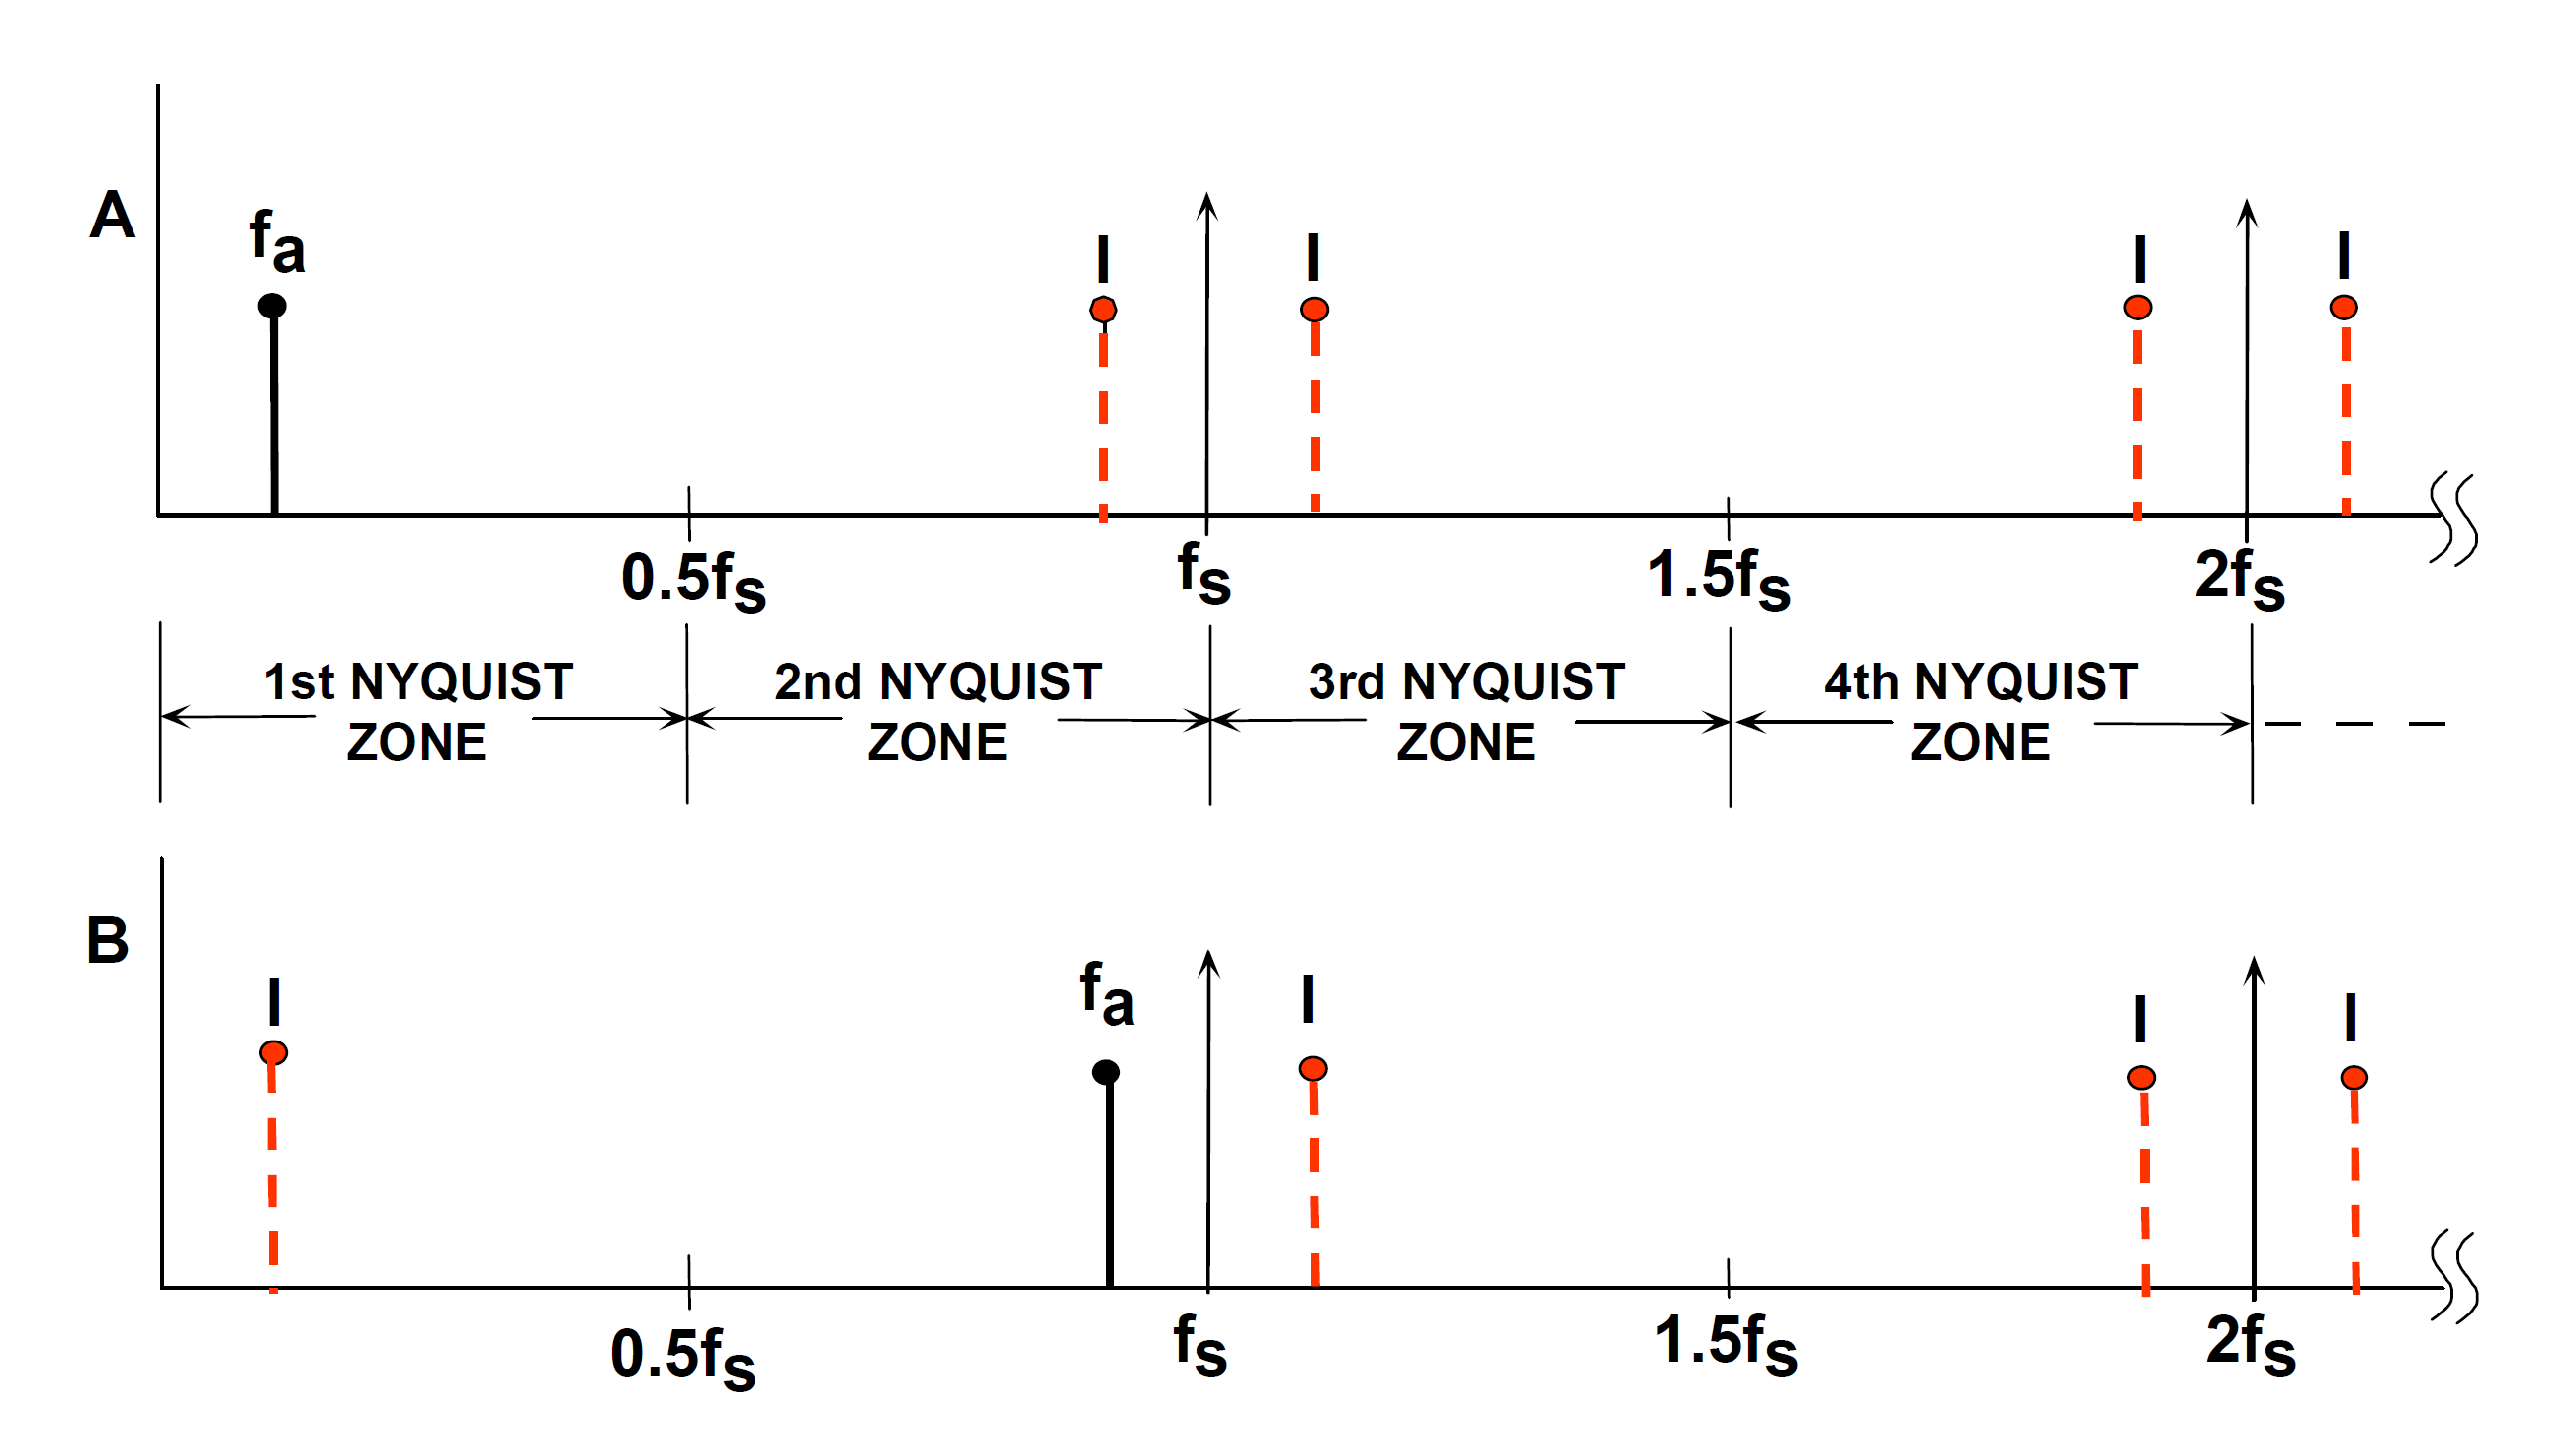
\includegraphics[width=\linewidth]{chap/02-theory/img/alias_f}  
		\caption{Sampling process visualized in frequency domain}
		\label{fig:alias_f}
	\end{subfigure}
	\begin{subfigure}{\textwidth}
		\centering
		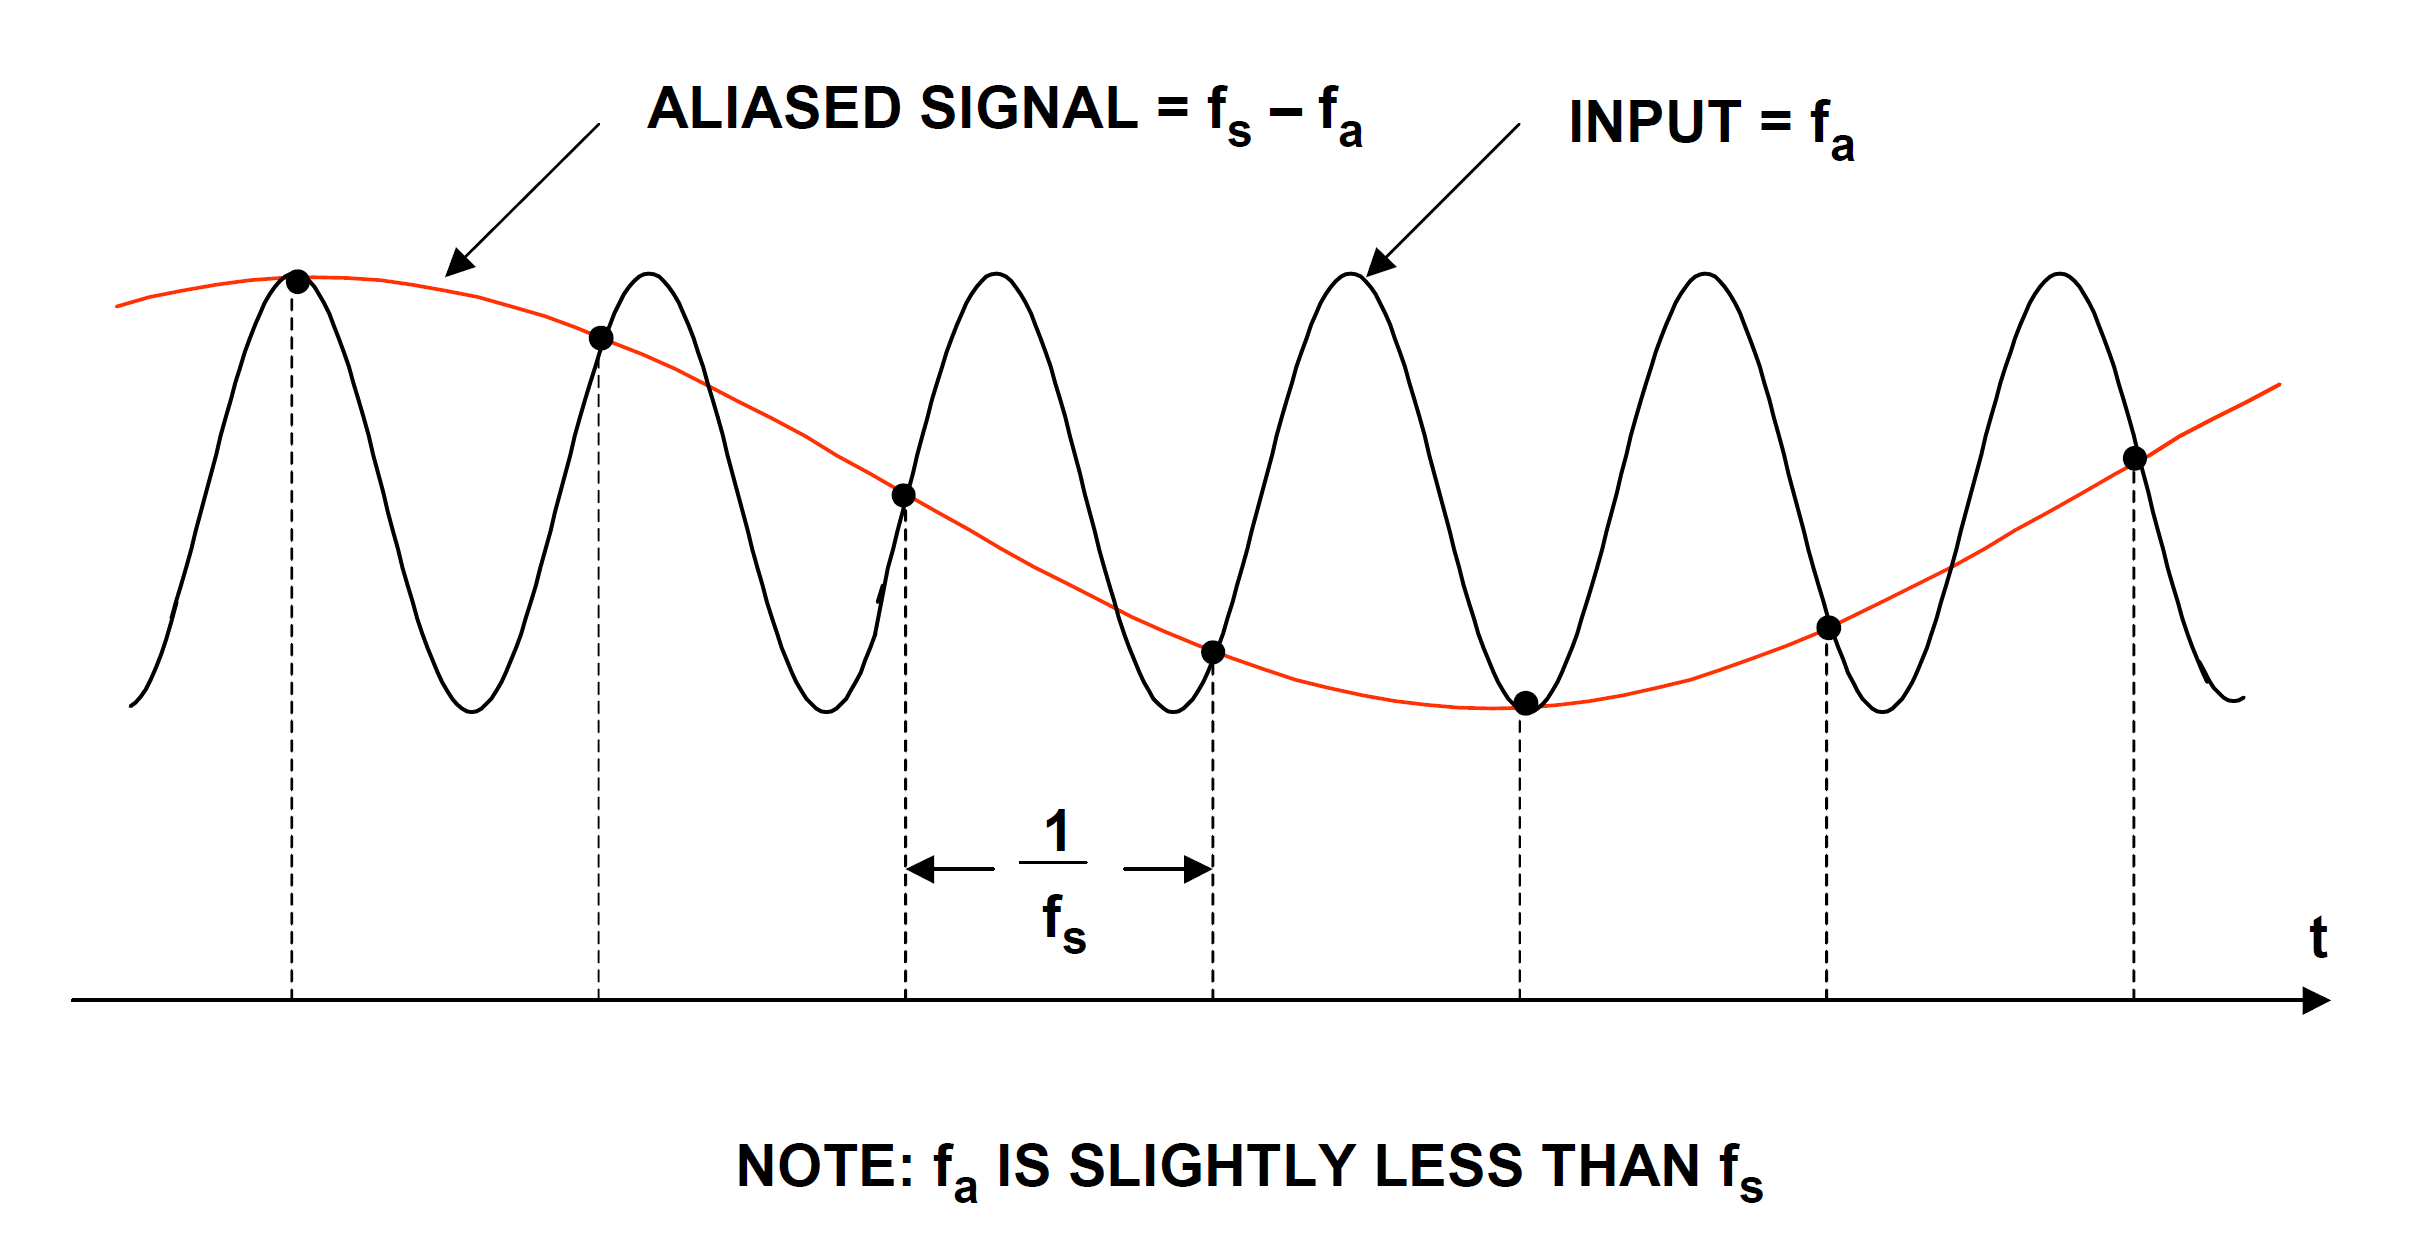
\includegraphics[width=\linewidth]{chap/02-theory/img/alias_t}  
		\caption{Effect of aliasing shown in time domain}
		\label{fig:alias_t}
	\end{subfigure}
	\caption[Aliasing]{Analog signal with frequency $f_a$ sampled at $f_s$ respecting (A) and not respecting (B) the Nyquist criteria (see \autoref{fig:alias_f}). \autoref{fig:alias_t} shows the effect of case B in time domain. \cite{walt}}
	\label{fig:aliasing}
\end{figure}
%todo low-pass filter to get B/2<f_s? maybe






    \chapter{Theoretical Fundamentals}
    		The main aspired use case of the newly developed time-stretch \gls{daq} lies in accelerator physics applications. Especially \gls{thz} science e.g. at \gls{kara} is of interest.
Therefore an introduction into this topic is given in the first section of this chapter. 

After that the general architecture and basic theory of a photonic time-stretch \gls{daq} is given.
First, the basic working principle of the time-stretch concept is explained.
Then, a short overview of the basic \gls{adc} theory is given, together with the most important figures of merit. 
Knowledge and understanding of \gls{adc} characteristics is necessary to evaluate the overall performance of the converter in the next chapters.

\section{Requirements in THz Science}
Recent years have seen an increasing interest in \gls{thz} radiation, ranging from \SI{3}{\tera \hertz} up to \SI{30}{\tera \hertz}\footnote{At \gls{kara}: \SIrange{0.1}{1.2}{\tera \hertz}}, as it allows non-destructive analysis of organic material. 
This is possible because unlike e.g. X-Rays, \gls{thz} radiation is not ionizing.
It is therefore of great interest to use \gls{thz} radiation in fields like biology, medicine or material science.
In biomedical research, \gls{thz} radiation has been used for spectroscopy, as energies involved in many biological processes lie in the terahertz frequency range. \cite{Bowen}
However, until recently the usage of \gls{thz} radiation was very limited, as generation of such radiation has proven to be difficult.

Synchrotrons and storage rings are a potential source of \gls{thz} radiation.
The emission of \gls{thz} radiation is closely linked to instabilities of the charged particles which are accelerated in a synchrotron (see \cite{mueller2012}). 
These instabilities occur in the time range of femtoseconds and cause bursts of \gls{thz} radiation.
The periodicity of these bursts depends on multiple parameters of the synchrotron and therefore imposes a challenge on controlling the emission of \gls{thz} radiation.
Studying the dynamics of these instabilities is an important step towards the application of synchrotrons as source of \gls{thz} radiation. \cite{rota2018}



\subsection{Coherent Synchrotron Radiation}
In synchrotron radiation facilities \gls{sr} is produced by accelerating relativistic electrons.
Emission of \gls{sr} occurs when electron beams are bent or deflected with dipole magnets or using undulators. The latter are used to make the electrons oscillate by generating a periodic magnetic field.  
\autoref{fig:storageRing} shows the general scheme of an electron storage ring.

Electrons, which are grouped to ``electron bunches'', are generated with an electron gun and accelerated to relativistic speeds\footnote{almost speed of light} by a pre-accelerator (often a \gls{linac}, a booster ring accelerator or a microtron with a booster). 
After being brought up to their nominal energy, the bunches are injected into the storage ring.
In the ring, the path of the electron bunches is altered by dipole magnets, guiding them on a circular trajectory.
Due to emission of \gls{sr} at each bend, the electrons lose energy, which has to be compensated for.
This is done by accelerating the electrons with an electric field inside a \gls{rf} cavity.
Not shown in the drawing are the beamlines, which lead the \gls{sr} radiation, or rather chosen wavelength ranges, through an optical system to the respective user experiments. \cite{roussel2014,rota2018}

\begin{figure}[tb]
	\centering
	\includegraphics[width=0.7\textwidth]{chap/02-theory/img/bd/synchrotron.pdf}
	\caption{Basic scheme of an electron storage ring (redrawn from \cite{roussel2014})}
	\label{fig:storageRing}
\end{figure}

The range of \gls{sr} reaches from hard X-rays down to the infrared region of the electromagnetic spectrum (see \autoref{fig:spectrum}).
\Gls{sr} shows properties like high intensity, high collimation, polarisation and generation in pulses of well-defined time duration.
High intensity is necessary for better penetration of the matter under study.
It prevents unnecessary exposure of the matter outside the area of interest and improves the image quality by producing less scatter radiation from these areas.
Well defined duration of the pulses allows to observe chemical reactions on short time scales.
Due to this properties, synchrotrons are used for microscopy, spectroscopy, and time-resolved experiments in such fields like condensed matter physics, biology, material science and many more. \cite{esrf}

\begin{figure}[tb]
	\centering
	\includegraphics[width = \textwidth, height = 0.5\textwidth]{chap/02-theory/img/bd/spectrum.tikz}
	\caption{Electromagnetic spectrum}
	\label{fig:spectrum}
\end{figure}

\clearpage
\paragraph{Karlsruhe Research Accelerator}
At the synchrotron light source \gls{kara}, the possibility to utilize a synchrotron as a source of \gls{thz} is actively researched. 
The photonic time-stretch \gls{daq}, which has been developed in this thesis, should also be integrated into the beam diagnostics system at \gls{kara}. 
Therefore, a short overview of some parameters of this facility is given below.

\gls{kara} is located at \gls{kit} and is operated by the \gls{ibpt}.
The storage ring can be filled up with up to 184 electron bunches with a distance of \SI{2}{\nano\second} ($\eqdev$ \SI{500}{\mega\hertz}) between two adjacent bunches.
The main accelerator parameters are listed in \autoref{tab:kara}. 

\begin{table}[tb]
	\caption{Some KARA parameters \cite{rota2018}}
	\label{tab:kara}
	\centering
	\begin{tabular}{ll}
		\toprule
		\textbf{Parameter}                  & \textbf{Value}                \\ \midrule
		Beam energy (max.)                  & \SI{2.5}{\giga \electronvolt} \\
		Circumference                       & \SI{110}{\meter}              \\
		Revolution Frequency (one electron) & \SI{2.7}{\mega \hertz}        \\
		        \multicolumn{2}{c}{\textbf{Minimum bunch spacing}}          \\
		\quad multi-bunch                   & \SI{2}{\nano \second}         \\
		\quad single-bunch                  & \SI{368}{\nano \second}       \\
		          \multicolumn{2}{c}{\textbf{Bunch length (rms)}}           \\
		\quad normal operation              & \SI{45}{\pico \second}        \\
		\quad short bunch                   & \SI{2}{\pico \second}         \\ \bottomrule
	\end{tabular}
\end{table}

One scientific focus at \gls{kara} lies in the study of so-called micro-bunching instabilitie' which are described next.

\subsubsection*{Micro-Bunching Instabilities}
Increasing demands in current and future accelerators applications call for higher brilliance of the emitted radiation. 
Brilliance denotes both the brightness and the angular spread of the beam. 
Higher brilliance allows to see more detail in the material under study. \cite{esrf}
The higher brilliance is achieved by shortening the electron bunches. 
As illustrated in \autoref{fig:csr}, this results in emission of \gls{csr}, the spectrum of which spans from \SI{100}{\GHz} up to \si{\tera \hertz}.
Due to this \gls{csr} the bunches interact with their own radiation as shown in \autoref{fig:electronInteract}, which introduces complex longitudinal dynamics. \cite{rota2018,brosi}

These dynamics are the so called micro-bunching instabilities: the formation of micro-structures (in the sub-millimeter range) in the longitudinal density profile of the electron bunches.
These instabilities occur in bursts and are hard to control, as they depend on a number of system parameters.
This imposes on one side a huge limitation to the stable operation of the overall system at high current density/short bunch length mode.
On the other side, these instabilities themselves emit brilliant \gls{thz} radiation that could be potentially used in imaging applications.
Such applications however require a stable power of the radiation. 
Therefore, a control of these instability bursts could potentially make them a source of \gls{thz} radiation for user-applications. 
A thorough understanding and studying of these beam dynamics is therefore an important step towards providing an applicable \gls{thz} source. \cite{rota2018,brosi}
In order to make such investigations possible, appropriate beam diagnostic systems are required, which are capable of both capturing (ultra-)fast and long-term changes in the bunch profile.  
\begin{figure}[tb]
	\centering
	\begin{subfigure}{0.4\textwidth}
		\centering
		\includegraphics[height=0.4\textwidth]{chap/02-theory/img/bd/SRincoherent.tikz}  
		\caption{Incoherent SR}
		\label{fig:srincoherent}
	\end{subfigure}
	\hfill
	\begin{subfigure}{0.4\textwidth}
		\centering
		\includegraphics[height=0.4\textwidth]{chap/02-theory/img/bd/SRcoherent.tikz}  
		\caption{Cohenrent SR}
		\label{fig:srcoherent}
	\end{subfigure}
	\begin{center}
		\begin{subfigure}{0.4\textwidth}
			\centering
			\includegraphics[width=1.2\textwidth]{chap/02-theory/img/bd/SRlegend.tikz}  
			\label{fig:srlegend}
		\end{subfigure}
	\end{center}
	\caption[Incoherent and coherent SR]{Incoherent \gls{sr} and coherent \gls{sr} due to shorter electron bunch length \cite{rota2018}}
	\label{fig:csr}
\end{figure}
\begin{figure}[tb]
	\centering
	\includegraphics[width = 0.8\textwidth]{chap/02-theory/img/bd/electronInteraction.tikz}
	\caption{Electrons interact with their own radiation \cite{Bielawski2019}}
	\label{fig:electronInteract}
\end{figure}
\subsection*{Control of Micro-Bunching Instabilities}
The \gls{ultrasync} project, funded by ANR-DFG\footnote{\gls{anr}, \gls{dfg}}, has an objective of ultrafast study and control of electron bunches in synchrotron light sources.

There is the question of control (i.e. suppression) of the bursts of \gls{thz} radiation occurring during the micro-bunching instability.
The goal is to obtain a high power and stable coherent emission. 
The current experimental setup uses a relatively simple feedback loop:
\begin{itemize}
	\item A bolometer/Schottky barrier diode detector which produces the input signal for the feedback loop.
	\item A low-cost \gls{fpga} that controls the the accelerating voltage of the synchrotron based on the input
\end{itemize}

However, there are limitations in the controllable bunch charge in the accelerator this feedback loop can handle, which is around \SI{10}{\milli \ampere}. 
Therefore, an open question is whether measuring each \gls{thz} pulse using the setup
\begin{itemize}
	\item \gls{eos} and time-stretching
	\item Association with the new \gls{fpga}-based system, i.e. \gls{theresa} system
	\item Finding adequate feedback, programmed in the \gls{fpga}
\end{itemize}
would help in solving the problem and allow the control to succeed also at higher currents (goal: \SI{15}{\milli \ampere}). \cite{bielwaski}

\subsection{Electro-Optic Techniques for Longitudinal Bunch Profile Diagnostics}
Methods for analyzing the longitudinal profile of electron bunches are based on a similar, if not the same, \gls{eo} concept as the time-stretch method. 
Two most prominent methods are briefly described for the sake of completeness.

\subsubsection*{Scanning-Type Electro-Optic Sampling}
The scanning-type \gls{eos} samples one point at the time of the \gls{thz} pulse, emitted e.g. from an electron bunch, at each acquisition, hence the naming of this method.

A short laser pulse (duration typically hundreds of femtoseconds) co-propagates with a \gls{thz} pulse from \gls{csr} (range of picoseconds) in an \gls{eo} crystal. 
Due to the Pockels effect the \gls{thz} pulse causes a time dependent birefringence in the crystal.
This modulates the polarization state of the laser pulse.

To sample the pulse, the delay between the laser and the \gls{thz} pulse is varied.
To detect the changing polarization, the polarization of the laser pulse is transformed into an intensity modulation. This is done by using polarizers, e.g. \glspl{qwp} and \gls{wp} (as shown in \autoref{fig:scan_eo}).
A general scheme of the system is shown in \autoref{fig:scan_eo}.
For this technique a stable emission of the \gls{thz} pulses is crucial, as they are not measured in one acquisition. \cite{roussel2014}
\begin{figure}[tbh]
	\centering
	%\includegraphics{chap/02-theory/img/bd/scan_eo.tikz}
	\resizebox{1\textwidth}{!}{\begin{tikzpicture}
	\node {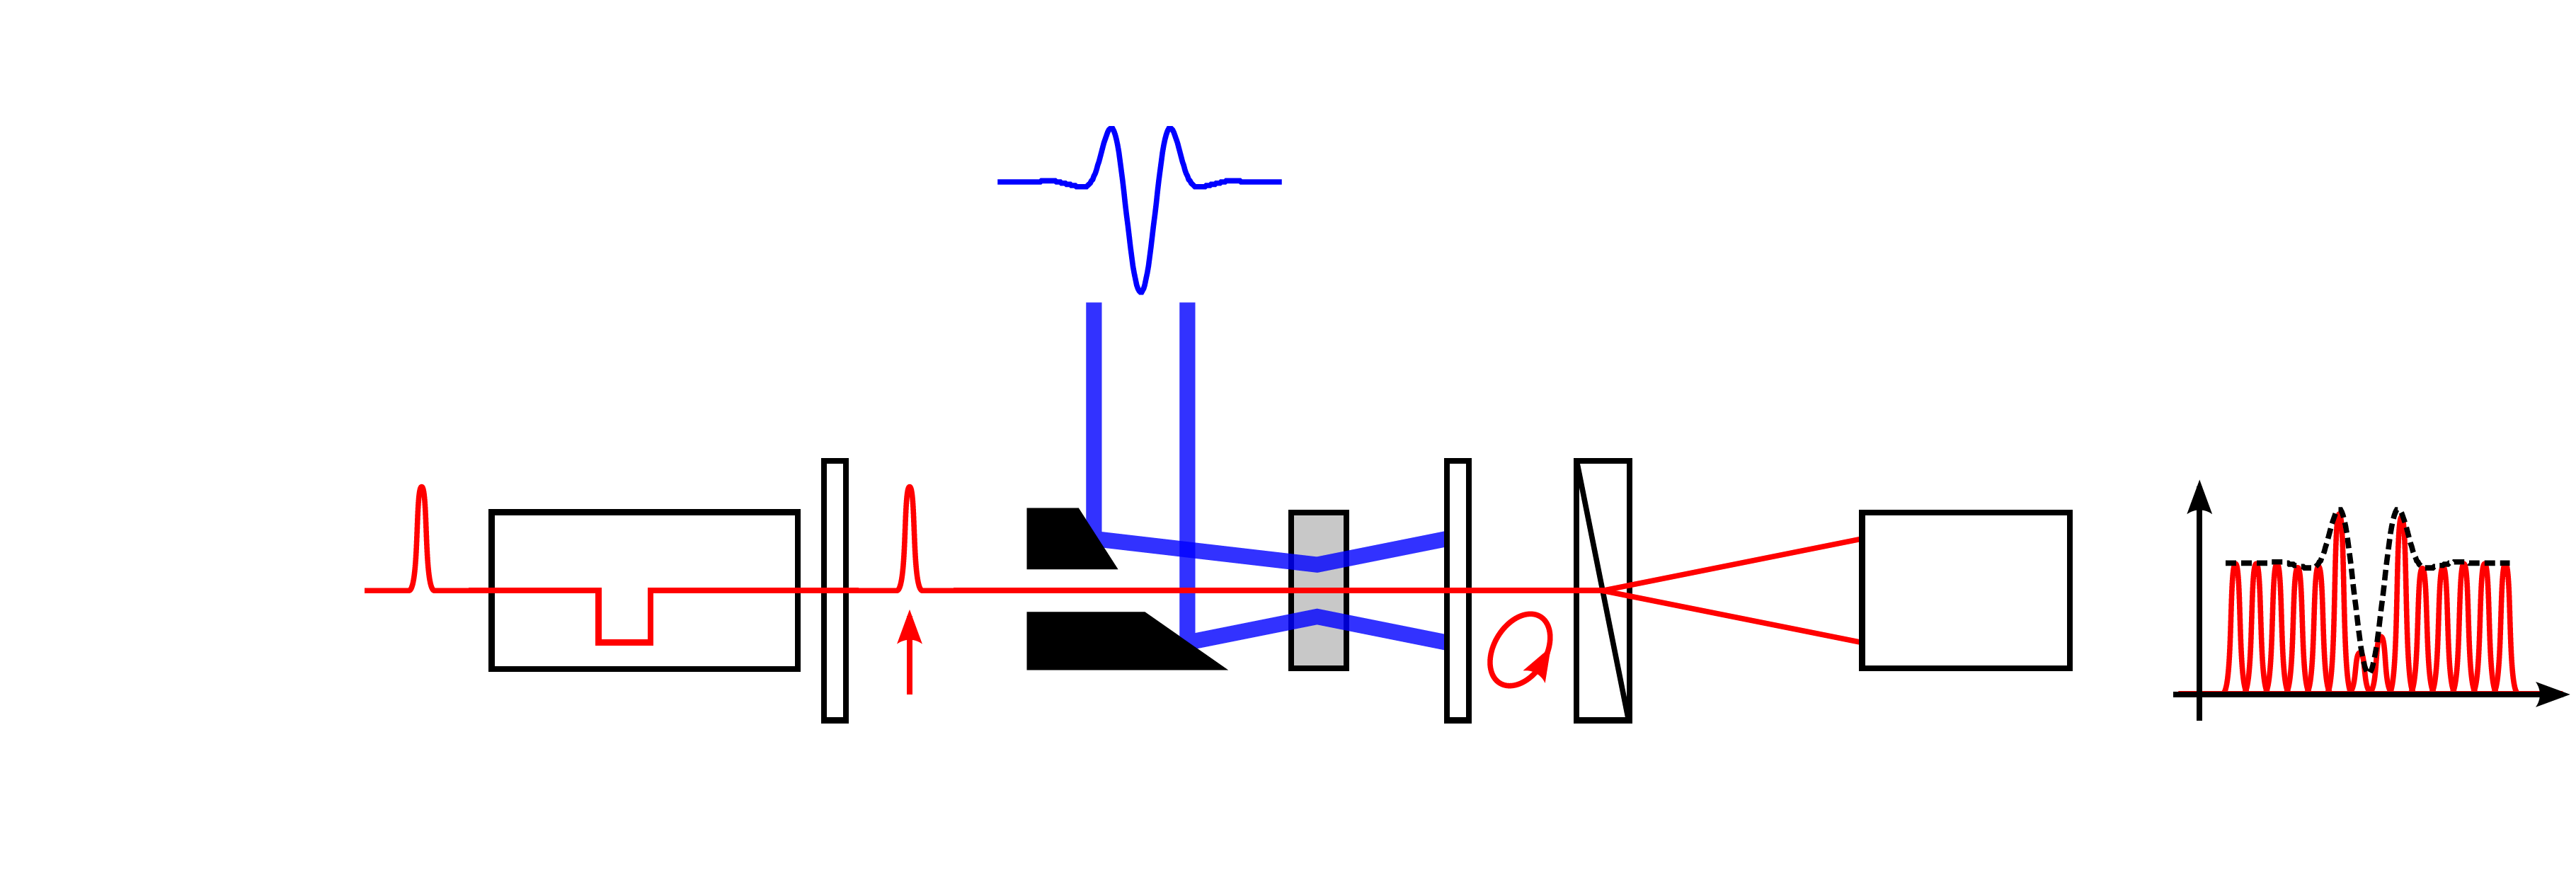
\includegraphics[width=10cm]{chap/02-theory/img/bd/scan_cleaned}};
	
	%left
	\node[fill=none,font=\tiny,align=right,anchor=east, align = center] at (-3.5,-0.4) {Short \\ laser pulse};
	\node[fill=none,font=\tiny,align=right,anchor=east] at (-1.9,-1.1) {Delay line};
	\node[fill=none,font=\tiny,align=right,anchor=east] at (-1.55,0.1) {P};
	\node[fill=none,font=\tiny,align=right,anchor=east] at (0.1,1.5) {THz pulse};
	\node[fill=none,font=\tiny,align=right,anchor=east, align = center] at (0.6,-1.3) {EO \\ crystal};
	\node[fill=none,font=\tiny,align=right,anchor=east] at (1.1,0.1) {QWP};
	\node[fill=none,font=\tiny,align=right,anchor=east] at (1.55,-1.3) {WP};
	\node[fill=none,font=\tiny,align=right,anchor=east] at (2,-0.25) {$I_1$};
	\node[fill=none,font=\tiny,align=right,anchor=east] at (2,-0.95) {$I_2$};
	\node[fill=none,font=\tiny,align=right,anchor=east, align = center] at (3.17,-0.6) {BD \\ $I_1 - I_2$};
	\node[fill=none,font=\tiny,align=right,anchor=east] at (5.1,-1.2) {Delay};
	\node[fill=none,font=\tiny,align=right,anchor=east] at (4,0) {Signal};
\end{tikzpicture}}
	\caption{Scheme of scanning-type electro-optical sampling system \cite{roussel2014}}
	\label{fig:scan_eo}
\end{figure}


\subsubsection*{Spectrally Resolved Electro-Optic Detection}
In contrast to the \gls{eos}, single-acquisition is possible with the spectrally resolved \gls{eo} detection technique.
The short laser pulse is first stretched to a duration similar to the \gls{thz} pulse in a dispersive material, called stretcher.
In this way the pulse is chirped, meaning the instantaneous frequency of the pulse varies over time.
Together with the \gls{thz} pulse, the laser pulse propagates through an \gls{eo} crystal.
Again, the induced birefringence modulates the laser pulse in time and in the spectral domain. 
The polarization state of the pulse is converted into an intensity modulation.
This is done with a series of \gls{qwp}, \gls{hwp} and a polarizer (P) (as shown in \autoref{fig:spectral_eo}).
To retrieve the \gls{thz} pulse shape in time, the spectrum of the laser pulse is measured with an optical spectrometer. 
A general scheme of the system is shown in \autoref{fig:spectral_eo}. \cite{roussel2014}

\begin{figure}[tbh]
	\centering
	%\includegraphics{chap/02-theory/img/bd/spectral_eo}
	\resizebox{1\textwidth}{!}{\begin{tikzpicture}
	\node {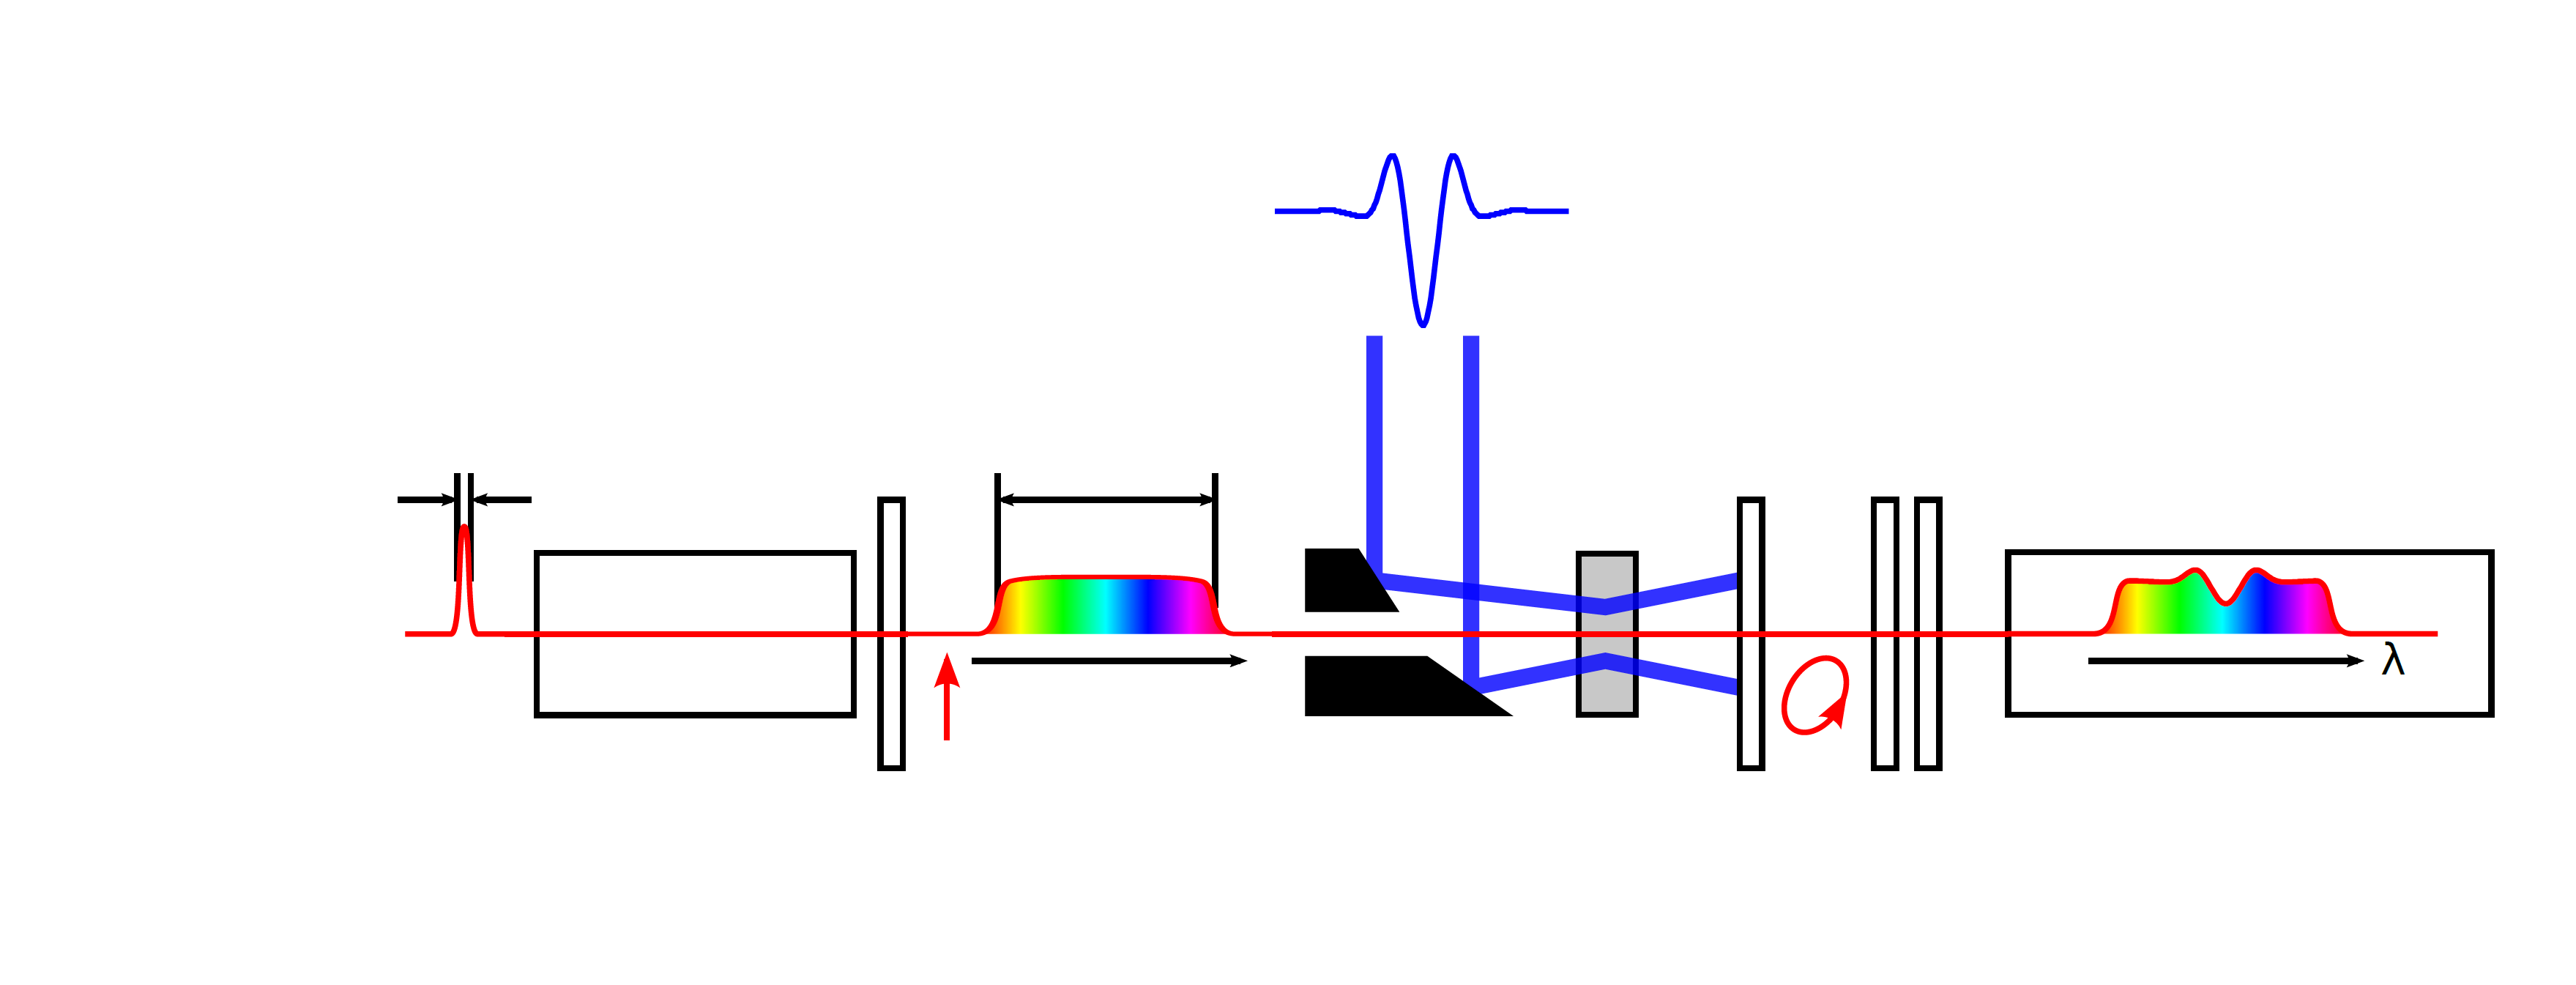
\includegraphics[width=10cm]{chap/02-theory/img/bd/spectral_eo_cleaned}};
	
	%left
	\node[fill=none,font=\tiny,align=right,anchor=east, align = center] at (-3.4,-0.4) {Short \\ laser pulse};
	\node[fill=none,font=\tiny,align=right,anchor=east] at (-2.8,0.2) {$T_0$};
	\node[fill=none,font=\tiny,align=right,anchor=east] at (-1.3,0.2) {P};
	\node[fill=none,font=\tiny,align=right,anchor=east] at (-0.3,0.2) {$T_c$};
	\node[fill=none,font=\tiny,align=right,anchor=east] at (-1.6,-1.1) {Stretcher};
	\node[fill=none,font=\tiny,align=right,anchor=east] at (0,-0.8) {Time};
	\node[fill=none,font=\tiny,align=right,anchor=east] at (1.2,1.5) {THz pulse};
	\node[fill=none,font=\tiny,align=right,anchor=east, align = center] at (1.7,-1.2) {EO \\ crystal};
	\node[fill=none,font=\tiny,align=right,anchor=east] at (2.2,0.1) {QWP};
	\node[fill=none,font=\tiny,align=right,anchor=east] at (2.7,0.1) {P};
	\node[fill=none,font=\tiny,align=right,anchor=east] at (2.9,-1.2) {HWP};
	\node[fill=none,font=\tiny,align=right,anchor=east] at (4.6,-1.1) {Spectrometer};
\end{tikzpicture}}
	\caption{Scheme of spectrally encoded electro-optical detection system \cite{roussel2014}}
	\label{fig:spectral_eo}
\end{figure}

The temporal resolution of this method is limited due to the finite chirp rate
\begin{equation}
	\text{chirp rate} = \frac{\text{laser bandwidth}}{\text{laser pulse duration after stretcher}}.
\end{equation}

The minimal resolution $T_{\text{min}}$ depends on the bandwidth-limited pulse duration (before stretcher) $T_0$ and the duration of the chirped laser pulse $T_c$ (see \cite{roussel2014}):
\begin{equation}
	T_{\text{min}} = \sqrt{T_0 T_c}
\end{equation}


\section{Photonic Time-Stretch Method}
The operating principle of the optical time-stretch technique can be described in three steps (see \autoref{fig:eo_ts}).

First, a short laser pulse (duration typically hundreds of femtoseconds) propagates in a dispersive medium, e.g. an optical fiber of length $L_1$ (see \autoref{fig:eo_ts}).
With the optical bandwidth of the laser pulse $\Delta \lambda$ and the dispersion parameter $D_1$ of the fiber, this results in a chirped laser pulse of the duration
\begin{equation}
	T_1 = \Delta \lambda D_1 L_1.
\end{equation}
The next step is the time-to-wavelength-mapping, where a temporal intensity modulation is imprinted on the chirped pulse.
This happens when the laser pulse co-propagates with another pulse, e.g. a \gls{thz} pulse from \gls{csr} (duration in the range of picoseconds), in an \gls{eo} crystal. 
Due to the Pockels effect the \gls{thz} pulse causes a time-dependent birefringence in the crystal. 
The Pockels effect describes the phenomenon of occurring and change of existing birefringence in an electric field, which is linearly proportional to the electric field strength. \cite{pockels} 

After that, the modulated chirped pulse propagates through another dispersive medium, a fiber of the length $L_2$.
In this way, the temporal modulation of the pulse is further stretched to the duration $T_2$, which is long enough for detection with photodetectors and the digitizing with \Glspl{adc}. \cite{roussel2014} 

The factor $M$, by which the pulse is slowed down, is calculated as (see \cite{roussel2014})
\begin{equation}\label{eq:ts}
	M = 1 + \frac{L_2}{L_1}.
\end{equation}
As example, assume the length of the dispersive media as $L_1 = \SI{10}{\meter}$ and $L_2 = \SI{2}{\kilo \meter}$ and an input signal with the duration $T_\text{sig} = T_1 = \SI{1}{\pico \second}$.
With \autoref{eq:ts} the stretching factor for this set-up is $M \approx 200$. The input pulse is stretched to $T_2 = M \cdot T_1 = 200 \cdot \SI{1}{\pico \second} = \SI{200}{\pico \second} = \SI{0.2}{\nano \second}$.
This corresponds to a frequency of $\SI{5}{\GHz}$ which is much easier to handle e.g. for an oscilloscope.
\begin{figure}[tb]
	\centering
	%\includegraphics{chap/02-theory/img/ts.tikz}
	\resizebox{1\textwidth}{!}{\begin{tikzpicture}
	\node {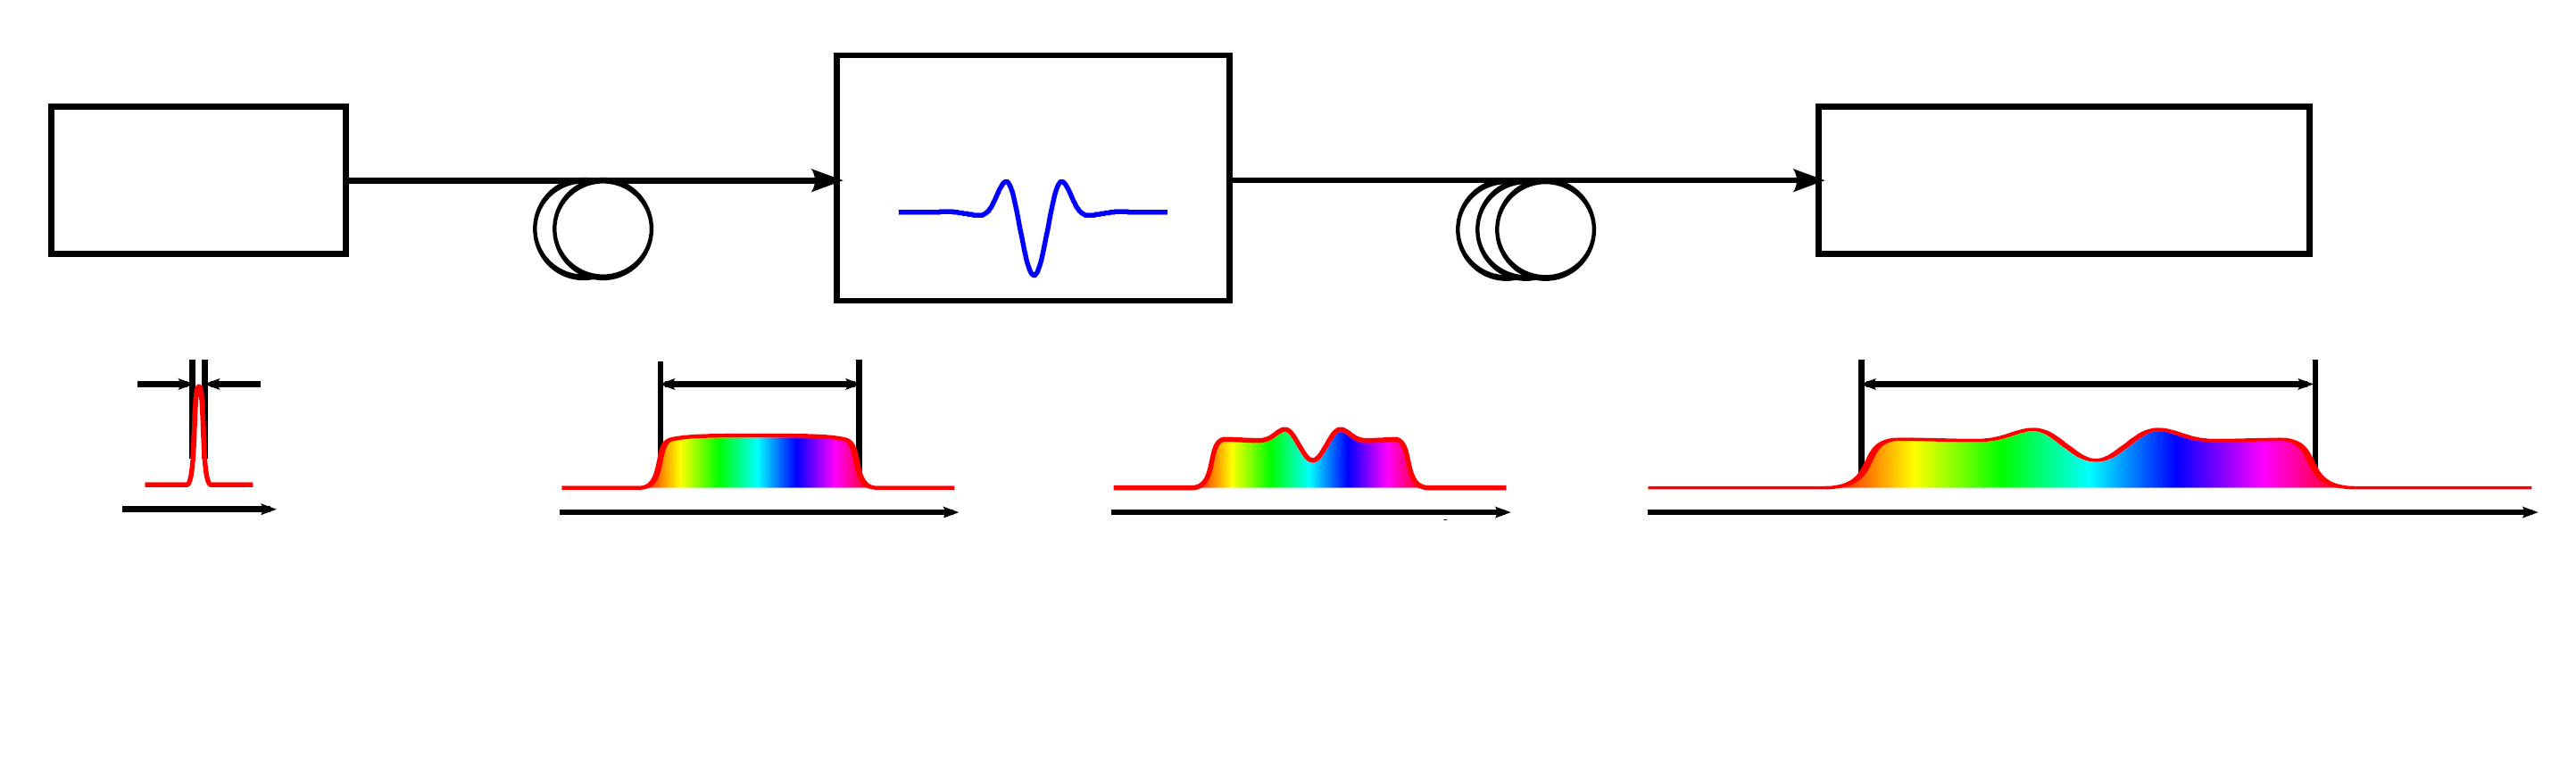
\includegraphics[width=10cm]{chap/02-theory/img/ts_cleaned}};
	
	%left
	\node[fill=none,font=\tiny,align=right,anchor=east] at (-3.8,0.78) {Laser};
	\node[fill=none,font=\tiny,align=right,anchor=east] at (-3.5,0) {$T_0$};
	\node[fill=none,font=\tiny,align=right,anchor=east] at (-3.5,-0.65) {\tiny Time};
	\node[fill=none,font=\tiny,align=right,anchor=east, align = center] at (-3.5,-1) {Short \\ laser pulse};
	\node[fill=none,font=\tiny,align=right,anchor=east] at (-1.2,-0.65) {\tiny Time};
	\node[fill=none,font=\tiny,align=right,anchor=east] at (-2,0.2) {Fiber $L_1$};
	\node[fill=none,font=\tiny,align=right,anchor=east] at (-2,1) {Dispersion};
	\node[fill=none,font=\tiny,align=right,anchor=east] at (-0.3,1) {Modulator};
	\node[fill=none,font=\tiny,align=right,anchor=east] at (1,-0.65) {\tiny Time};
	\node[fill=none,font=\tiny,align=right,anchor=east] at (-1.3,0) {$T_1$};
	\node[fill=none,font=\tiny,align=right,anchor=east, align = center] at (-1.4,-1) {Chirped \\ laser pulse};
	\node[fill=none,font=\tiny,align=right,anchor=east] at (5,-0.65) {Time};
	\node[fill=none,font=\tiny,align=right,anchor=east, align = center] at (1.4,-1) {Time-to-wavelength\\ mapping};
	\node[fill=none,font=\tiny,align=right,anchor=east] at (1.6,0.2) {Fiber $L_2$};
	
	
	\node[fill=none,font=\tiny,align=right,anchor=east] at (4.1,-0.9) {Stretched signal};
	\node[fill=none,font=\tiny,align=right,anchor=east] at (4.5,0) {$T_2$};
	\node[fill=none,font=\tiny,align=right,anchor=east] at (3.9,0.78) {Photodetector};
\end{tikzpicture}}
	\caption{Working principle of the electro-optical time-stretch technique \cite{roussel2014}}
	\label{fig:eo_ts}
\end{figure}

\paragraph{Photodetector}
In order to convert the time-stretched optical signal into an electrical value, a photodetector, e.g. a photodiode, is needed.
A circuit is a photo-diode operated in reverse bias, meaning the $p$-side is connected to the negative terminal and the $n$-side to the positive terminal of a power supply with some sort of current-limiting capability.
This enlarges the depletion region (see \autoref{fig:pn_junc}) of the $p/n$-junction as the depletion region contains only a very small amount of free charge carriers. 
Irradiating the diode with photons of sufficient energy generates electron-hole pairs due to the photoelectric effect.
If the electron-hole pairs are produced in the depleted region of the $p/n$-junction, they are separated by the electric field applied across, before they can recombine. 
This creates a so called photo-current which can be measured and converted into a voltage signal. \cite{photodiode}

\begin{figure}[tbh]
	\centering
	\includegraphics[]{chap/02-theory/img/pn.tikz}
	\caption{pn-junction with depleted region \cite{pn-junc}}
	\label{fig:pn_junc}
\end{figure}

\newpage
\section{Analog-To-Digital Converter}
\Glspl{adc} are used to translate analog signals, like voltages, into the digital representation of these signals.
This \textit{digitized} version can then be stored and processed by information processing, computing, data transmission and control systems. 
This translation, also called ``conversion'', can be seen as encoding a continuous-time analog input $V_\text{in}$(t) (voltage) into a series of discrete, $N$-bit words. 
This process is also called \textit{sampling}. 
With the full-scale voltage of $V_{\text{FS}}$, which denotes the maximal output voltage of the \gls{adc}, the individual output bits $b_k$ and the quantization error $\epsilon$ (see \autoref{par:quant_noise}), the \gls{adc} should satisfy the relation (see \cite{Lundberg})
\begin{equation} \label{eq:adc_sample}
	V_{\text{in}}(t) = V_{\text{FS}} \sum_{k = 0}^{N-1} \frac{b_k}{2^{k+1}} + \epsilon.
\end{equation}
This can also be rewritten in terms of the \gls{lsb}, or quantum level $V_Q$, (see \cite{Lundberg})
\begin{equation}
	1 \; \text{LSB} = \frac{V_\text{FS}}{2^N} = V_Q.
\end{equation}
With \autoref{eq:adc_sample} this leads to 
\begin{equation}
	V_\text{in} = V_Q \sum_{k = 0}^{N-1} b_k 2^{k}  + \epsilon.
\end{equation}

\autoref{fig:idealADC} shows the ideal transfer function of a 3-bit \gls{adc}. 
Each digital $N$-bit word corresponds to a range of input voltage values (\textit{code width}), which is centered around a \textit{code center}. \cite{Lundberg}
The input voltage is resolved to the code of the nearest code center.
\begin{figure}[H]
	\centering
	\includegraphics[width = 0.7\textwidth]{chap/02-theory/img/adc/ideal_adc.tikz}
	\caption[Transfer function of ideal, 3-bit ADC]{Transfer function of an ideal, 3-bit \gls{adc} (redrawn from \cite{Lundberg})}
	\label{fig:idealADC}
\end{figure}

\clearpage
\paragraph{Sample-And-Hold-Amplifier}
\Glspl{adc} need a certain amount of time to sample the input signal.
If the level of the analog signal changes by more than one \gls{lsb} during this period, this can result in large errors in the output signal.
Therefore so called \gls{sha} are used in front of the \gls{adc} to hold the input level constant for the needed amount of time. \cite{walt}

It consists of an input and output unity gain amplifier, a switch controlled by the sampling clock and a capacitor.
The analog input passes through the input unity gain amplifier which leads to a switch that is controlled by a sampling clock.
During the sample mode, i.e. during the negative sampling clock cycle, the switch is open.
At the transition from negative to positive clock cycle, the switch closes, connecting the input signal with the capacitor which is charged in this way and buffers the input signal. \cite{walt} 

The \gls{adc} sampling time needs to be timed in such way, that the whole duration of an analog-to-digital conversion falls into the hold period of the \gls{sha} and does not exceed into the sample period. 
\autoref{fig:sha_timing} shows a qualitative example for proper sample timing. 
As conclusion, the upper frequency limitation is not determined by the \gls{adc} itself, but rather by the aperture jitter, bandwidth, distortion, etc. of the \gls{sha}. \cite{walt}

\begin{figure} [tbh]
	\centering
	\tikzexternaldisable
	\includegraphics[width=\linewidth]{chap/02-theory/img/adc/sha_timing.tikz}  
	\tikzexternalenable
	\caption[SHA timing example]{Example for appropriate sampling timing when using Sample-And-Hold-Amplifier. The sample points of the \gls{adc} should be inside the period, where the \gls{sha} holds the input value.}
	\label{fig:sha_timing}
\end{figure}

\paragraph{Track-And-Hold Amplifier}
Apart from the \glspl{sha} there also exists the so called \gls{tha}. 
A general block diagram of a \gls{tha} is shown in \autoref{fig:tha_low}.
Though the names are often used interchangeably, there is one fundamental difference between a \gls{sha} and a \gls{tha}.
Strictly speaking, the output of a \gls{sha} is not defined during the sample period. 
Only when switching to the hold mode, the output is assigned to a defined value: the voltage level at the input in that moment.
Contrary to that, the \gls{tha} acts as a unity gain amplifier during the sample period, meaning the output is just a replication of the input. 
The \gls{tha} ``tracks'' the input signal (see also \autoref{fig:tha_up}).
Therefore, instead of speaking of a ``sample'' period, the term used here is the ``track'' period.
When switching to hold mode, the instantaneous input level is held over the course of the hold period.
This principle allows to improve the sampling rate, as the settling time of an \gls{tha} is in general smaller than the one of a \gls{sha}.
Settling time denotes the amount of time needed for the output voltage to be at a stable level, after the transition from track/sample to hold mode.
This process is quicker, when the output voltage is already in the range of the sampled input at the moment, instead of when the hold capacitor first has to be charged to the input voltage. \cite{Reeder2017}

\begin{figure}[tbh]
	\centering
	\begin{subfigure}{\textwidth}
		\centering
		\includegraphics[width=0.85\textwidth]{chap/02-theory/img/adc/tha_low.tikz}  
		\caption{Schematic of a THA}
		\label{fig:tha_low}
	\end{subfigure}
\\[4ex]
	\begin{subfigure}{\textwidth}
		\centering
		\includegraphics[height=0.6\textwidth, width = 0.9\textwidth]{chap/02-theory/img/adc/tha_up.tikz}  
		\caption{Working principle of the THA}
		\label{fig:tha_up}
	\end{subfigure}
	\caption{Track-And-Hold-Amplifier schematic and principle \cite{walt}}
	\label{fig:tha_principle}
\end{figure}

\subsection{Characteristics of Analog-To-Digital-Converters}\label{ssec:adc_charac}
For an ideal converter, the number of bits and the sampling rate would be sufficient to fully characterize its performance.
Real \glspl{adc} however differ from the ideal behavior by introducing static and dynamic imperfections.
Different applications have different requirements, which leads to a number of specifications.
These can be divided into the categories according to \cite{Lundberg}:
\begin{itemize}[noitemsep]
	\item Quantization Noise
	\item Static parameters
	\item Frequency-domain dynamic parameters
	\item Time-domain dynamic parameters
\end{itemize} 
This section provides an overview of these figures of merit.
Which of them are needed to specify the necessary performance of the \gls{adc} has to be chosen for each application accordingly.

\subsubsection{Quantization Noise}\label{par:quant_noise}
Even an ideal $N$-bit converter has errors resulting from the quantization process which can be modeled like noise. 
The reason is that each $N$-bit word represents a certain range of analog input values, which is 1 \gls{lsb} wide and centered around a code center (see \autoref{fig:idealADC}). \cite{Lundberg}

The input voltage is assigned to the word of the nearest code center.
This means that there will always be a difference between the corresponding voltage of the respective digital code $x_q(t)$ and the actual analog input voltage $x(t)$.
This difference is called the \textit{quantization error}. For an equidistant quantization, the quantization error for a code width $q$ is (see \cite{puente2015})
\begin{equation}
	\left| e_q(t) \right| = \left| x(t) - x_q(t) \right| \leq \frac{q}{2}.
\end{equation}
A setup in order to measure this quantization error is shown in \autoref{fig:qe_m}. 
\begin{figure}[tb]
	\centering
	\includegraphics[width = 0.8\textwidth]{chap/02-theory/img/adc/quant_err_meas.tikz}
	\caption[Measurement setup for quantization error]{Setup for measuring the quantization error of an (ideal) \gls{adc} with input signal $x(t)$}
	\label{fig:qe_m}
\end{figure}

The output of the \gls{adc}, the $N$-bit code corresponding to the voltage level of the input signal $x(t)$, is fed to a \gls{dac}, which converts this code into a corresponding voltage level $x_q(t)$. 
The difference between $x(t)$ and $x_q(t)$ is the quantization error $e_q(t)$.

In order to analyze the quantization noise and the resulting theoretical maximum \gls{snr} of the ideal \gls{adc}, assume a ramp with the slope $s$ as an input signal. 
Then, the quantization error $e_q(t)$ can be approximated with a sawtooth signal in the time domain (see \cite{walt}): 
\begin{equation}\label{eq:qe_saw}
	e_q(t) = st, \quad -\frac{q}{2s} < t < \frac{q}{2s} 
\end{equation}
The function in \autoref{eq:qe_saw} is plotted in \autoref{fig:eq}.
\begin{figure}[tb]
	\centering
	\includegraphics[width = 0.7\textwidth]{chap/02-theory/img/adc/quantization_error.tikz}
	\caption{Quantization noise as function of time (redrawn from \cite{walt})}
	\label{fig:eq}
\end{figure}

The power of this quantization noise can be calculated as the mean-square $e_{\text{rms}}^2$ of $e(t)$ (see \cite{walt}):
\begin{equation}
	P_\text{QN} = e_{\text{rms}}^{2} = \overline{e^{2}(t)} = \frac{s}{q}\int_{-q/2s}^{+q/2s} (st)^{2} dt = \frac{s^3}{q} \left[ \frac{t^3}{3}\right]_{-\frac{q}{2s}}^{+\frac{q}{2s}} = \frac{q^2}{12}
\end{equation}

In order to calculate the maximal \gls{snr} of an ideal converter, a full-scale input sine wave is applied to the input:
\begin{equation}
	u(t) = u_s \sin(2\pi f t) = \frac{2^{N}q}{2}\sin(2\pi f t)  = 2^{N-1}q \sin(2\pi f t)
\end{equation}
With the effective value of the signal amplitude
\begin{equation}
	u_{\text{eff}} = \frac{u_s}{\sqrt{2}} = \frac{2^{N-1}q}{\sqrt{2}}
\end{equation}
the \gls{snr} can be calculated as 
\begin{equation}
	\text{SNR} = \frac{P_{\text{signal}}}{P_{\text{noise}}} = \frac{u_{\text{eff}}^{2}}{e_{\text{rms}}^{2}} = \frac{2^{2N-2}q^2/2}{q^2/12} = 2^{2N} \cdot 1.5.
\end{equation}
In decibel, the \gls{snr} is calculated as (see \cite{puente2015, walt}):
\begin{equation}\label{eq:idealSNR}
	\text{SNR}|_{\text{dB}} = 10\log\left(2^{2N}\cdot 1.5\right) = 6.02 N + 1.76
\end{equation}

\clearpage
\subsubsection{Static parameters}
\textit{Static parameters} are specifications, which can be measured at low speed/DC. 
\paragraph{Accuracy}
\textit{Accuracy} is the total error with which an \gls{adc} can convert a known voltage, which includes the effects of (see \cite{Lundberg}):
\begin{itemize}[noitemsep]
	\item Quantization error
	\item Gain error
	\item Offset error
	\item Non-linearities
\end{itemize}

\paragraph{Resolution}
\textit{Resolution} is the number of bits $N$ of the \gls{adc}.
Depending from the resolution are the size of the \gls{lsb}, which in its turn determines the dynamic range, code widths and quantization error.
\paragraph{Dynamic Range}
The \textit{dynamic range} represents the ratio between smallest possible output (\gls{lsb} voltage) and the largest possible output (full-scale voltage).
It can be calculated as
\begin{equation}
	20 \log 2^{N} \approx 6N.
\end{equation}

\paragraph{Offset and Gain Error}
The \textit{offset error} is defined as the deviation of the actual \gls{adc} transfer function from the ideal \gls{adc} transfer function in the point of zero. It is measured in \gls{lsb}. 

\textit{Gain Error} defines the deviation of the slope of the line going through the zero and full-scale point of the transfer function.
\autoref{fig:offsetErr} visualizes the effects of both offset and gain error. 
\begin{figure}[tbh]
	\centering
	\includegraphics[width = 0.8\textwidth]{chap/02-theory/img/adc/adc_offset_gain.tikz}
	\caption[Effects of Offset and Fain error in ADC]{Offset and Gain Error in the \gls{adc} characteristic transfer function. The offset error is indicated with the red arrow. The gain error expresses itself via different slope of the real \gls{adc} (dotted) compared to the ideal \gls{adc} (dashed)}
	\label{fig:offsetErr}
\end{figure}

These errors can easily be corrected by calibration. 
In order to measure the offset and gain error, two different voltage levels $V_1$ and $V_2$ are applied at the \gls{adc} input. 
This results in corresponding bit codes $b_1$ and $b_2$.
The slope $s$ of the transfer function can then be calculated by
\begin{equation}
	s = \frac{b_2 - b_1}{V_2 - V_1}.
\end{equation}
From this, the gain error can be determined.
In order to obtain the offset error $b$, the linear equation
\begin{equation}
	b = b_1 - s\cdot V_1
\end{equation}
is solved.

\paragraph{Integral and Differential Non-Linearity Distortion} 
\gls{inl} is the distance of the code centers on the actual \gls{adc} transfer function from the ideal line (dashed line in \autoref{fig:nld}). 
It results from the integral non-linearities of the front-end, \gls{sha} and also the \gls{adc} itself \cite{walt, Lundberg}. 

\gls{dnl} is the deviation in actual code width from the ideal width of 1 \gls{lsb}. This non-linearity stems exclusively from the encoding process in the \gls{adc}. \cite{Lundberg,walt}

The effect of these errors is shown in \autoref{fig:nld}.
\begin{figure}[tbh]
	\centering
	\includegraphics[width = 0.8\textwidth]{chap/02-theory/img/adc/nonlinear.tikz}
	\caption[ADC Non-linearities]{Transfer function of a real \gls{adc} showing \gls{dnl} and \gls{inl} \cite{Lundberg}}
	\label{fig:nld}
\end{figure}

These non-linearities could be measured with a histogram test.
A voltage ramp is applied at the input and the number of occurrences of each \gls{adc} output code, $n(\text{code})$, is measured.
With the ramp slope $s$ ([s] = \si{\volt \per \second}) of an ideal \gls{adc} with the sampling frequency $f_s$ would give (see \cite{inlDnl})
\begin{equation}
	n(\text{code}) = \frac{\text{LSB}}{s} \cdot f_s = n_\text{avg},
\end{equation}
which ideally would be constant for the whole input range (except for the first and last code).
For a real \gls{adc} this is not the case and the \gls{dnl} and \gls{inl} are calculated as (see \cite{inlDnl})
\begin{align}
	\text{DNL(code)} &= \frac{n(\text{code})-n_\text{avg}}{n_\text{avg}}\\
	\text{INL(code)} &= \sum_{i = 0}^{\text{code}} \text{DNL}(i).
\end{align}


\subsubsection{Frequency-Domain Dynamic Parameters}
Any real \gls{adc} is subject to noise distortion. 
\textit{Noise} denotes any unwanted random signal, which interferes with the measuring of the desired signal. 
Examples are quantization noise or random fluctuations due to thermal noise. 
\textit{Distortion} is the term for alteration of the shape of the original signal. 
As an example, distortion of the amplitude might result due to not equal amplification of the parts of a signal. \cite{wiley}

In an \gls{adc} (with built-in \gls{sha}) there are a couple of sources, which introduce noise and distortion:
\begin{itemize}
	\item \textbf{Input Stage:} Wideband noise, non-linearity and bandwidth limitation
	\item \textbf{\gls{sha}:} Non-linearity, aperture jitter (see \autoref{ssec:time_param}) and bandwidth limitation 
	\item \textbf{\gls{adc}:} Quantization noise, non-linearity
\end{itemize}

For quantification of noise and distortion, frequency-domain metrics are used. 
Therefore the figures of merit described in the following paragraphs are also called frequency-domain dynamic parameters. 
These parameters are measured with the help of the \gls{fft} meaning any modern oscilloscope can be used to quickly assess the frequency-domain dynamic performance for a given input at the \gls{adc}.
As some parameters, such as \gls{sfdr}, are only defined for one carrier input frequency, several measurements at different input frequencies need to be carried out in order to fully characterize the \gls{adc}.

In the following paragraphs, an overview of the metrics for quantification of the noise and distortion of an \gls{adc} is given. 


\paragraph{Signal-to-Noise Ratio}
The \gls{snr} is defined as the ratio of the input signal power to the power of the noise signal. 
It is expressed in \si{\dB} and can be calculated using the \gls{rms} value of the signal and noise amplitudes (see \cite{xilinx_adc}):
\begin{align}
	\text{SNR} & = \frac{\text{Power}_\text{Signal}}{\text{Power}_\text{Noise}}                                    \\
	           & = \left( \frac{\text{Amplitude}_\text{Signal, rms}}{\text{Amplitude}_\text{Noise, rms}} \right)^2 \\
	           & = 20 \log \left( \frac{V_\text{in, rms}}{V_\text{Q, rms}}\right)
\end{align}
Usually, the \gls{snr} degrades at higher frequencies due to sampling jitter. \cite{xilinx_adc}

\paragraph{Signal-to-Noise-and-Distortion Ratio}
\gls{sinad} (also called SNDR or S/N+D) denotes the ratio between the \gls{rms} of the signal amplitude to the mean value of the \gls{rss} of all other spectral components, including harmonics, but excluding \gls{dc} (\SI{0}{\hertz}). 
\gls{sinad} is a good indication over the general dynamic performance of the \gls{adc}, as it includes all contributions from noise and distortion.
The higher the \gls{sinad} the stronger the input power is differentiated from noise and spurious components. \cite{xilinx_adc} 

\gls{sinad} can be calculated from the average power of the input signal $P_\text{signal}$, noise $P_\text{noise}$ and $P_\text{distortion}$ (see \cite{xilinx_adc}):
\begin{equation}
	\text{SINAD} = 10 \log \left( \frac{P_\text{signal}}{P_\text{noise} + P_\text{distortion}} \right)
\end{equation}
It is commonly expressed in dB, \gls{dbc} or \gls{dbfs}.

\paragraph{Effective-Number-Of-Bits}
The \gls{enob} expresses the \gls{sinad} in terms of bits. It can be calculated as (see \cite{walt2009}):
\begin{equation}
	\text{ENOB} = \frac{\text{SINAD}-\SI{1.76}{\decibel}}{\SI{6.02}{\decibel \per \bits}}. 
\end{equation}
This is derived from solving the equation of the ``ideal \gls{snr}'' (\autoref{eq:idealSNR}) for the number of bits $N$ and substituting \gls{snr} with \gls{sinad}.
This however means, that this parameter assumes a full-scale input signal. Expressing the \gls{enob} for a smaller signal amplitude requires measuring the \gls{sinad} at this level and a correction factor. \cite{walt}

\paragraph{Spurious-Free Dynamic Range}
\gls{sfdr} indicates the dynamic range of the converter, which can be used, before there is interference or distortion from spurious components with the fundamental signal. \cite{Lundberg} 
The \gls{sfdr} is calculated as the \gls{rms} value of the fundamental signal to the \gls{rms} value of the worst spurious signal, i.e. the highest spur in the spectrum.
It is measured over the whole Nyquist bandwidth from \gls{dc} to $\nicefrac{f_s}{2}$, with $f_s$ being the \gls{adc} sampling rate. The spur may or may not be a harmonic of the fundamental signal. \cite{walt2009, Lundberg}

The \gls{sfdr} is an important characteristic in the sense, that it indicates the smallest signal which can still be distinguished from a strong interfering signal. \cite{walt2009} 

The \gls{sfdr} in \gls{dbc} can be calculated as (see \cite{xilinx_adc}):
\begin{equation}
	\text{SFDR}_\text{dBc} = 20 \log \left( \frac{\text{Fundamental Amplitude (RMS)}}{\text{Largest Spur Amplitude (RMS)}} \right).
\end{equation}


\autoref{fig:sfdr} illustrates the \gls{sfdr} in terms of \gls{dbfs} and \gls{dbc}.

\begin{figure}[tbh]
	\centering
	\includegraphics[width = \textwidth]{chap/02-theory/img/adc/sfdr.tikz}
	\caption[SFDR definition]{Visualization of the \gls{sfdr}. It can be indicated either with reference to the carrier frequency in ``dBc'' or with reference to the Full-Scale Input in ``dBFS''. \cite{walt2009}}
	\label{fig:sfdr}
\end{figure}

\paragraph{Total Harmonic Distortion}
\textit{Total Harmonic Distortion} describes the ratio of the \gls{rms} sum of the first five harmonic components (or aliased versions of them) to the \gls{rms} of the considered fundamental signal. \cite{Lundberg}

\paragraph{Effective Resolution Bandwidth}
\textit{Effective Resolution Bandwidth} denotes the frequency of the input signal, at which the \gls{sinad} has fallen by \SI{3}{\decibel} ($\eqdev$ 0.5 bit in terms of \gls{enob}) compared to the \gls{sinad} at lower frequency range. \cite{Lundberg}

\paragraph{Analog Input Bandwidth}
\textit{Analog Input Bandwidth} is the analog input frequency at which the power of the fundamental component is reduced by \SI{3}{\dB} with respect to the low-frequency value. \cite{Lundberg}
It is not to be confused with the maximal input frequency which the \gls{adc} is able to sample.

\paragraph{Full-Linear Bandwidth}
The \textit{Full-Linear Bandwidth} is defined as the frequency at which the slew-rate of the \gls{sha} starts to distort the input signal by a specified value. \cite{Lundberg} 
The slew-rate (SR) is defined as the rate of how much the voltage $V(t)$ changes over time $t$:
\begin{equation}
	\text{SR} = \frac{\text{d}V(t)}{\text{d}t}
\end{equation}

A slew-rate of \SI{1}{\volt \per \micro \second} for example means, that the output of the amplifier can not change more than \SI{1}{\volt} over the course of \SI{1}{\micro \second}. \cite{2021Slew} 

\subsubsection{Time-Domain Dynamic Parameters}\label{ssec:time_param}
Time-Domain Dynamic parameters describe the deviation of the converter's behavior from the ideal one in time domain. 

\paragraph{Aperture Delay}
\textit{Aperture Delay} (or \textit{aperture time}) is defined as delay between the triggering of the converter (e.g. rising edge of the sampling clock) and the actual conversion of the input voltage into the digitized value. \cite{Lundberg}

\paragraph{Aperture Jitter}
\textit{Aperture jitter} describes the sample-to-sample variation in aperture delay.
Jitter can cause significant error in the voltage and decreases the overall \gls{snr} of a converter.
Especially for high-speed \glspl{adc} jitter poses a limit in performance.

Assuming a full-scale sine wave $V_{\text{in}}$(t) as input signal with 
\begin{equation}
	V_{\text{in}}(t) = V_{\text{FS}} \sin(\omega t)
\end{equation}
the maximal slope of this signal is then
\begin{equation}
	\frac{\text{d}V_{\text{in}}(t)}{\text{d}t}\Bigr|_{\text{max}} = \omega V_{\text{FS}}
\end{equation}
Aperture jitter $\Delta t_{\text{rms}}$ occurring during the sampling of this maximal slope produces the \gls{rms} voltage error 
\begin{equation}
	\Delta V_{\text{rms}} = \omega  V_{\text{FS}} \Delta t_{\text{rms}} = 2 \pi f  V_{\text{FS}} \Delta t_{\text{rms}}.
\end{equation}
As variations in aperture time occur randomly, these errors behave like a random noise source.
This way, a \gls{sjnr} can be defined as
\begin{equation}
	\text{SJNR} = 20 \log \left( \frac{V_{\text{FS}}}{\Delta V_{\text{rms}}} \right) = 20 \log \left( \frac{1}{2 \pi f  V_{\text{FS}}} \right)
\end{equation}

The voltage error due to jitter and the \gls{sjnr} for different aperture jitter values are shown in \autoref{fig:ap_jit}.

\begin{figure}[tbh]
	\centering
	\begin{subfigure}{0.45\textwidth}
		\centering
		\includegraphics[width = \textwidth,height=1\textwidth]{chap/02-theory/img/adc/jitterTimeDomain.tikz}  
		\caption{Effect of aperture jitter}
		\label{fig:jitter}
	\end{subfigure}\hfill
	\begin{subfigure}{0.45\textwidth}
		\centering
		\includegraphics[width = \textwidth,height=1\textwidth]{chap/02-theory/img/adc/SJNRjitter.tikz}  
		\caption{SJNR for different aperture jitter values}
		\label{fig:sjnr}
	\end{subfigure}
	\caption[Aperture jitter and SJNR]{Effects of aperture jitter on the output voltage and SJNR. Left: In time domain, Right: SJNR for different aperture jitter \cite{Lundberg}}
	\label{fig:ap_jit}
\end{figure}

\paragraph{Transient Response}
The \textit{transient response} denotes the settling time of an \gls{adc} until full accuracy ($\pm$ 1/2 \gls{lsb}).


\subsubsection{Sampling Theory}
An \gls{adc} samples an analog signal with a sample frequency $f_s$.
This frequency has to be chosen in such way, that the original signal can be fully reconstructed.
The \textit{Nyquist criteria} states, that in order to accurately reconstruct continuous signal limited to the bandwidth $B$ (see \cite{puente2015})
\begin{equation}
	y (t) \, \laplace \,  Y(f) \quad \text{with} \quad Y(f)=0\vert_{f>B/2}
\end{equation} 
it has to be sampled with a frequency $f_s$ respecting
\begin{equation} \label{eq:nyquist}
	f_s > B \quad \text{or} \quad f_s > 2 f_a,
\end{equation}
with $f_a$ being the highest frequency contained in the signal. \cite{walt,puente2015}

The range from \SI{0}{\Hz} to $\nicefrac{f_s}{2}$ is also called \textit{Nyquist-Zone} (or ``1st Nyquist zone'', see \autoref{fig:alias_f}).
Violation of this rule leads to \textit{aliasing}.
The effects of aliasing are shown in \autoref{fig:alias}.

When a harmonic wave of the frequency $f_a$ is sampled with the frequency $f_s$, this leads to periodic repetition of the signal spectrum in frequency domain in intervals of $f_s$, or ``images'' (see dashed, red frequency components in \autoref{fig:sampling}). 
If \autoref{eq:nyquist} is respected, i.e. $f_a$ lies inside the Nyquist bandwidth, there is no overlap with the images created by the sampling process.

Now assuming a signal frequency $f_a \approx f_s$, the sampling process leads to an image falling inside the Nyquist bandwidth (see \autoref{fig:alias_f}).
The reconstructed signal then lies at the frequency of this image which is much lower than the original frequency.
The result of this \textit{undersampling} is shown in \autoref{fig:alias_signal}. \cite{nyquist, shannon, walt}
\begin{figure}[tbh]
	\centering
	\begin{subfigure}{0.9\textwidth}
		\centering
		\includegraphics[width=\textwidth]{chap/02-theory/img/adc/sampling.tikz}  
		\caption{Analog signal with frequency $f_a$ sampled at $f_s$ respecting the Nyquist criteria}
		\label{fig:sampling}
	\end{subfigure}
	\\[4ex]
	\begin{subfigure}{0.9\textwidth}
		\centering
		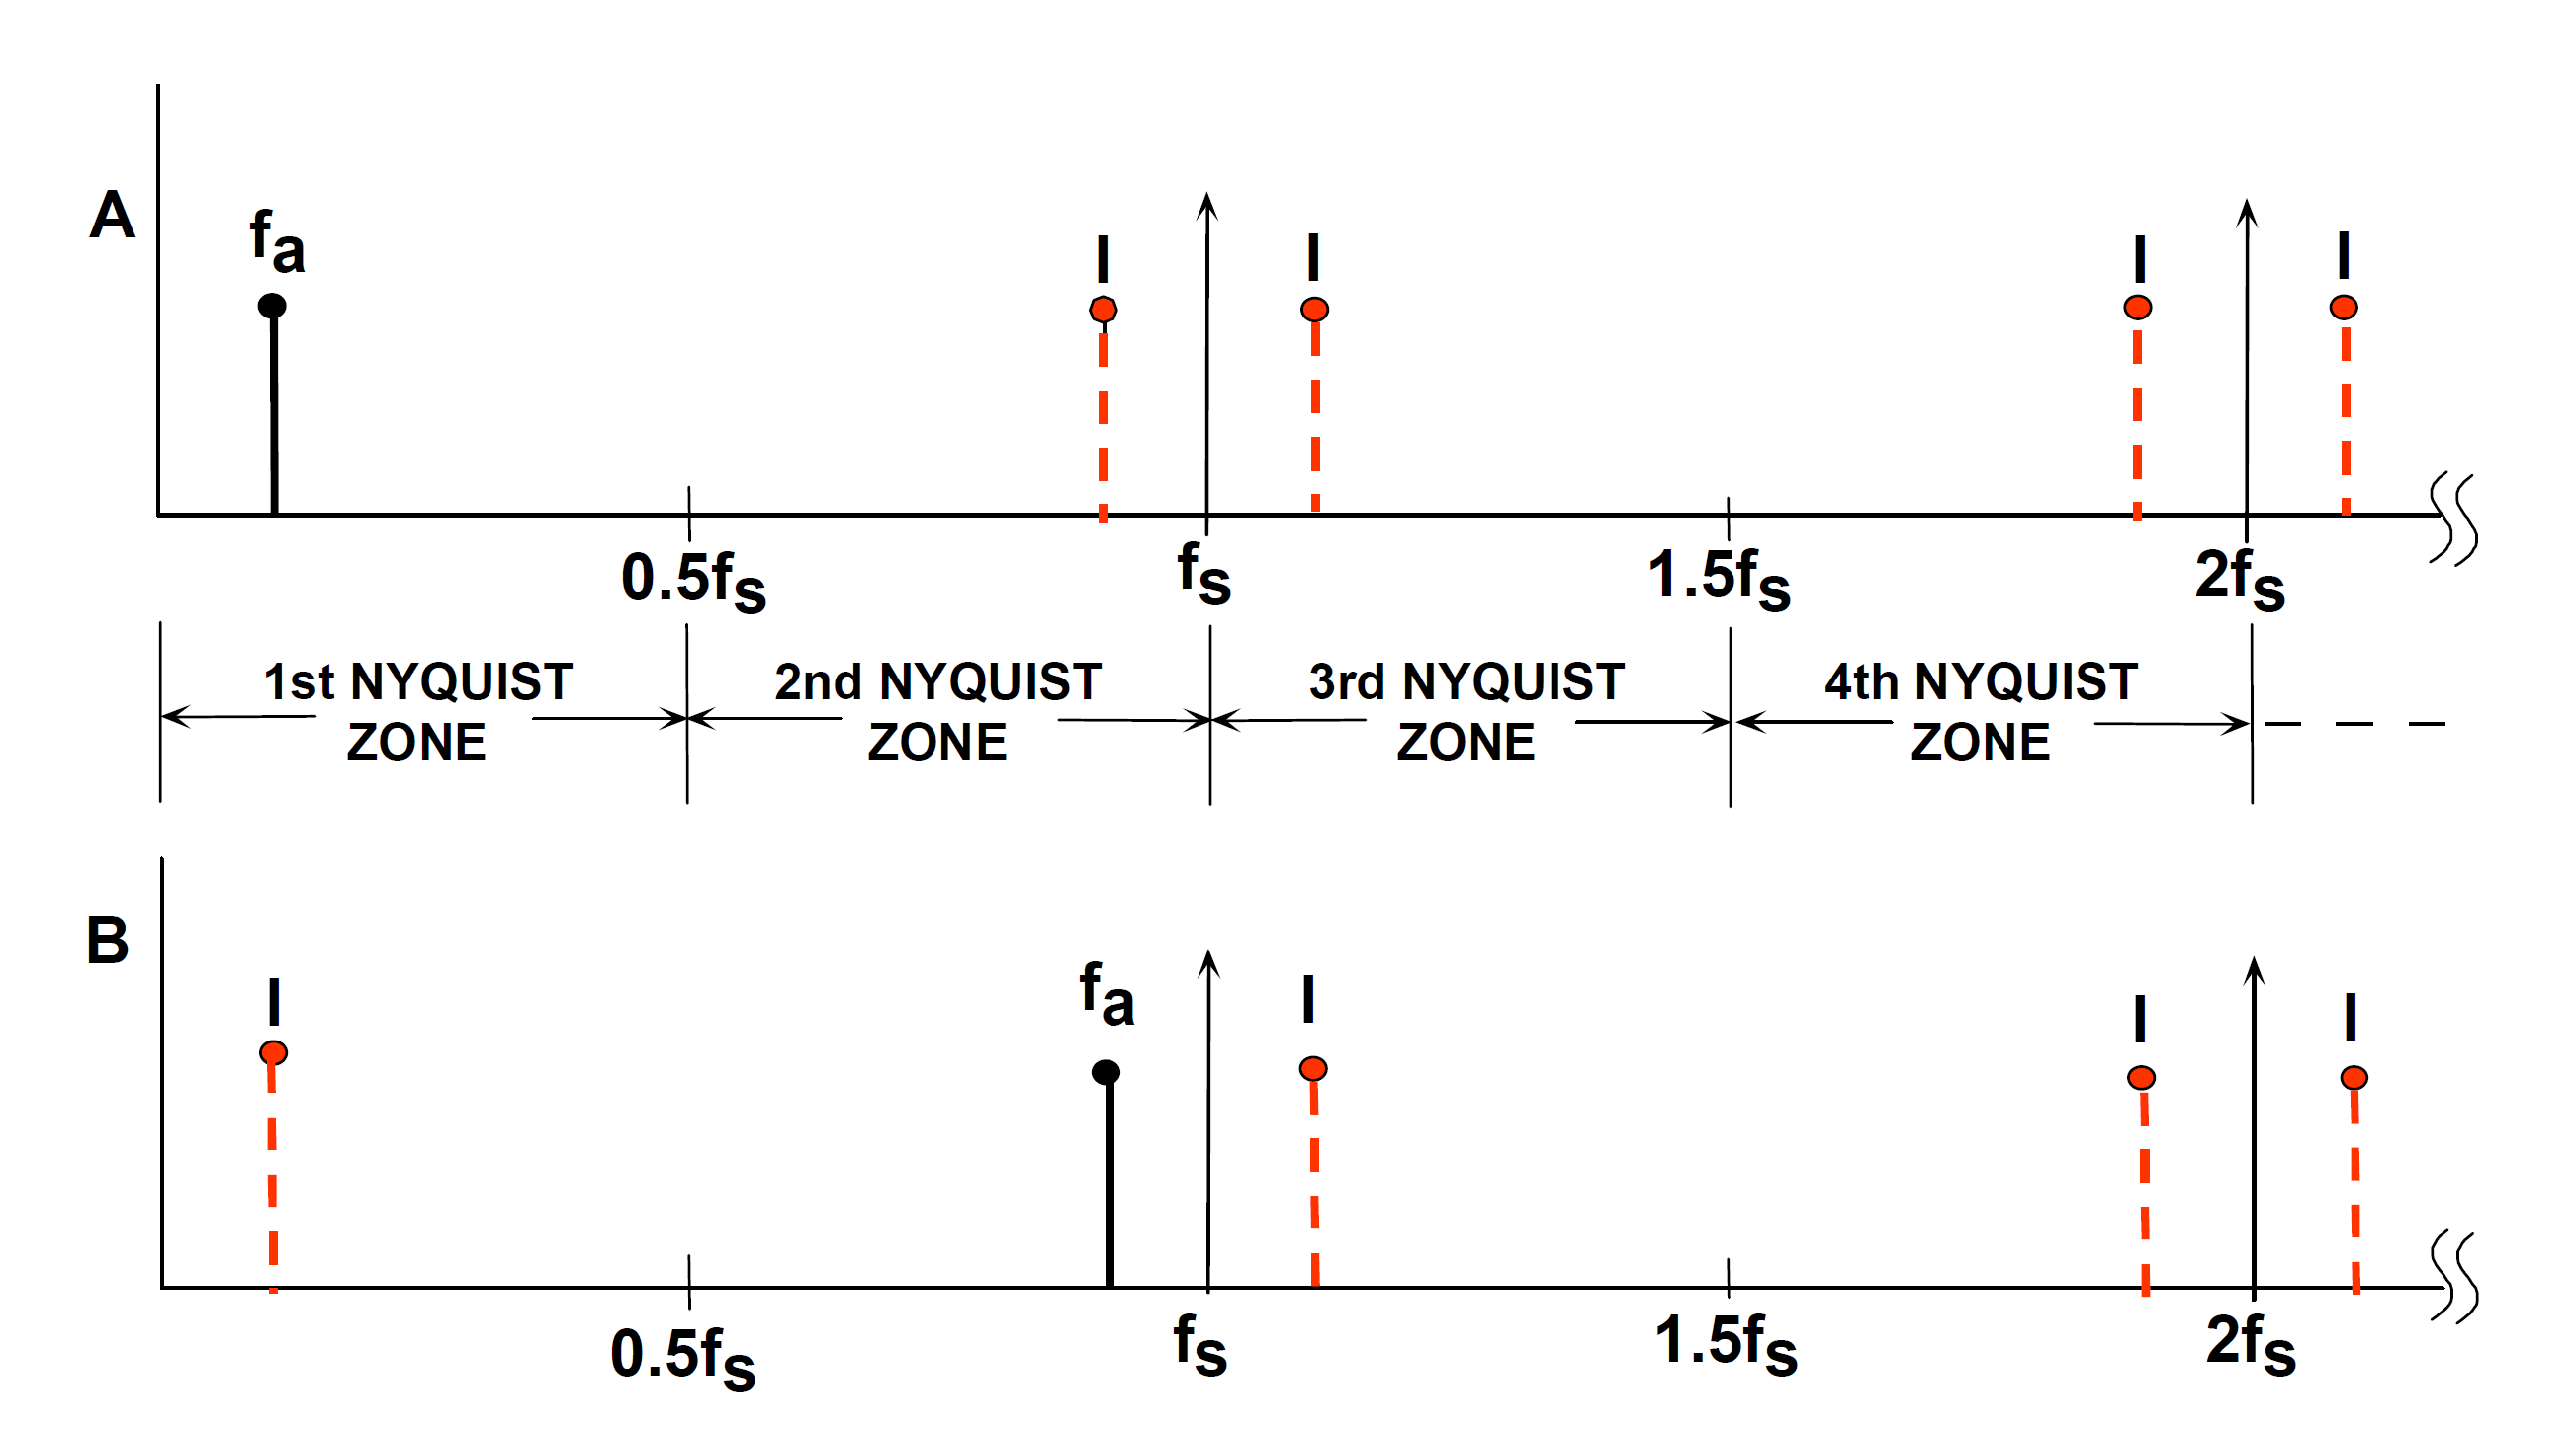
\includegraphics[width=\textwidth]{chap/02-theory/img/adc/alias_f.tikz} 
		\caption{Analog signal with frequency $f_a$ sampled at $f_s$ not respecting the Nyquist criteria}
		\label{fig:alias_f}
	\end{subfigure}
	\\[4ex]
	\begin{subfigure}{\textwidth}
		\centering
		\includegraphics[height=0.5\textwidth, width = \textwidth]{chap/02-theory/img/adc/alias.tikz}  
		\caption{Effect of aliasing in time domain}
		\label{fig:alias_signal}
	\end{subfigure}
	\caption[Aliasing]{Analog signal with frequency $f_a$ sampled at $f_s$ respecting (\autoref{fig:sampling}) and not respecting (\autoref{fig:alias_f}) the Nyquist criteria. \autoref{fig:alias_signal} shows the effect of aliasing in time domain. \cite{walt}}
	\label{fig:alias}
\end{figure}




	\chapter{Design of the system}
			This chapter covers the architecture and design of the system.
\section{General architecture}
In this section the general architecture of the THERESA system is described.
The idea for the new system is to reuse the concept of the already existing sampling system KAPTURE (\textbf{Ka}rlsruhe \textbf{P}ulse \textbf{T}aking \textbf{U}ltra-fast \textbf{R}eadout \textbf{E}lectronics), which is using four ADCs, and expanding it to 16. Therefore, also the architecture of the latter is explained briefly.
\subsection{KAPTURE-2}
KAPTURE, which was developed at IPE, is a system designed to continuously sample ultra-short pulses generated by Terahertz detectors. It consists of a daughter card, holding four sampling channels, mounted on a FPGA . The FPGA is connected to a computer via PCIe for further processing of the acquired data. \cite{brosi} 
The newer version, KAPTURE-2, was designed for more accurate sampling for pulse repetition rates up to \SI{2}{\giga \hertz}. The acquired data is processed with a FPGA and GPU architecture.  \cite{caselleKAP}

The general structure of the board is shown in \autoref{fig:kapture}.

\begin{figure}[H]
	\centering
	\includegraphics[width = \textwidth]{chap/03-work/img/kapture.tikz}
	\caption{General schema of KAPTURE-2 (cf. \cite[p.2]{caselleKAP})}
	\label{fig:kapture}
\end{figure}


The pulse from the \SI{}{\tera \hertz} detector is fed into a power splitter, which splits the signal into four identical pulses and distributes them to four channels, consisting of a respective Track-And-Hold-Amplifier (THA) unit and a 12-bit ADC@\SI{500}{\mega\sample\per\second}. The sampling time of each unit can be adjusted individually with a Picosecond Delay Chip with a resolution of \SI{3}{\pico \second} (maximal delay range: \SI{100}{\pico \second}). 
The clock signal is provided by KARA, which is cleared from jitter by a Phase-Locked-Loop (PLL). This ensures the synchronization of the ADCs with the RF system. The clean clock signal is distributed to the delay chips via fan-out. \cite{caselleKAP}

The resulting sampling of the detector signal is shown \autoref{fig:detector_signal} (simplified representation).
\begin{figure}[H]
	\centering
	\includegraphics[height = 0.3\textwidth, width = 0.6\textwidth]{chap/03-work/img/detector_signal.tikz}
	\caption{Signal with sample points}
	\label{fig:detector_signal}
\end{figure}

\begin{figure}[H]
	\centering
	\includegraphics[width = 0.8\textwidth]{chap/03-work/img/kapture_sys}
	\caption{Photo of KAPTURE with highlighted main components. \cite[p.~61]{brosi}}
	\label{fig:kapturesys}
\end{figure}

\newpage
\subsection{New System THERESA}
In principle, the new system has the same structure, as KAPTURE. Notable differences are firstly the number of ADCs, which is increased up to 16. Secondly, the latter are not located on the daughter card anymore, but inside the Xilinx Zynq UltraScale+ RFSoC ZU49DR on the ZCU216 Evaluation Kit on which the front-end card is mounted. \autoref{fig:theresa_scheme} shows the general schema of the sampling system, reduced to four channels for presentation purposes.
\begin{figure}[H]
	\centering
	\includegraphics[width = \textwidth]{chap/03-work/img/theresa_scheme.tikz}
	\caption{General schema of THERESA. For presentation purposes only four channels are shown.}
	\label{fig:theresa_scheme}
\end{figure}

\paragraph{Xilinx Zynq UltraScale+ RFSoC ZCU216 Evaluation Card}
The card, holding the sampling channels, should be mounted on a ZCU216 evaluation board. This board is the newest generation of Xilinx' evaluation cards, which has features suitable for the purpose at hand.
\begin{itemize}[noitemsep]
\item Sixteen 14-bit, 2.5GSPS RF-ADC
\item Sixteen 14-bit, 10GSPS RF-DAC
\item I/O expansion options – FPGA Mezzanine Card (FMC+) interfaces, RFMC 2.0 interfaces, and Pmod connections
\end{itemize}
\begin{figure}[H]
	\centering
	\includegraphics[width = \textwidth]{chap/03-work/img/zcu216}
	\caption{ZCU216 evaluation board}
	\label{fig:zcu216}
\end{figure}
 
\begin{figure}[H]
	\centering
	\includegraphics[width = 0.6\textwidth]{chap/03-work/img/rfsoc_blockdiagram}
	\caption{RFSoC block diagram}
	\label{fig:rfsoc}
\end{figure}

\subsection{Requirements}
\paragraph{Step size delay chip}
The necessary step size for the delay chips, when using 16 ADC@\SI{2}{\giga \sample \per \second} in time-interleaving mode, is: $\frac{\SI{2}{\giga \sample \per \second}}{16} = \SI{31}{\pico \second}$

\paragraph{Frequency}


\begin{figure}[H]
\centering
\tikzexternaldisable
\begin{tikztimingtable}
  TH1 & 1H 8L N(A1) 8L 16H \\
  TH2 & 2H 16L 15H \\
  TH3 & 3H 16L 14H \\
  TH4 & 4H 5L N(B1) 11L 13H \\
  \\
  TH5 & 5H 16L 12H \\
  TH6 & 6H 16L 11H \\
  TH7 & 7H 16L 10H \\
  TH8 & 8H 16L 9H \\
  \\
  TH9 & 9H 16L 8H \\
  TH10 & 10H 16L 7H \\
  TH11 & 11H 16L 6H \\
  TH12 & 12H 16L 5H \\
  \\
  TH13 & 13H 16L 4H \\
  TH14 & 14H 16L 3H \\
  TH15 & 15H 16L 2H \\
  TH16 & 16H 16L 1H \\
\extracode
 \tablerules
 \begin{pgfonlayer}{background}
 \draw [help lines, dashed] (A1) -- (B1);
 \end{pgfonlayer}
\end{tikztimingtable}
\tikzexternalenable
\caption{Track-And-Hold Timing diagram}
\label{fig:THA}
\end{figure}




\paragraph{Data Rate}
\paragraph{Visualization/GUI}
\newpage
\section{Design of the front-end card}
In this section, the design of the front-end card is covered.

\subsection{Sampling-Channel}
\paragraph{Track-And-Hold-Amplifier}
Explain why better than Sample-And-Hold-Amplifier.
\paragraph{Delay Chip NB6L295}
Dual Channel Programmable Delay Chip.

\begin{itemize}[noitemsep]
	\item Two individual variable delay channels
	\item Dual Delay: minimal delay \SI{3.2}{\nano \second}
	\item Total Delay Range: \SI{3.2}{\nano \second} to \SI{8.8}{\nano \second} per Delay Channel
	\item \SI{11}{\pico \second} Increments in 511 steps
	\item \SI{100}{\pico \second} Typical Rise and Fall Times
\end{itemize}

\subsection{Clocking}
On Xilinx CLK104 add-on board the LMX2594 is used to generate additional, high-frequency clocks for the ADCs/DACs. $\rightarrow$ reuse in front-end card
\begin{figure}[H]
	\centering
	\includegraphics[width = 0.7\textwidth]{chap/03-work/img/clk104}
	\caption{CLK104 Add-on board clocking scheme}
	\label{fig:clk104}
\end{figure}

\begin{figure}[H]
	\centering
	\includegraphics[height = 0.3\textwidth, width = 0.55\textwidth]{chap/03-work/img/pll_tsMode.tikz}
	\caption{Clocking scheme on front-end card}
	\label{fig:clocking}
\end{figure}


\begin{figure}[H]
	\centering
	\includegraphics[width = 0.7\textwidth]{chap/03-work/img/pll.png}
	\caption{Placeholder}
	\label{fig:pll}
\end{figure}



\subsection{Power Supply}
For the Track-And-Hold amplifiers a new power supply unit -- the ADP1741 (Analog Devices) -- should be used. It is necessary to think about the amount of power supply chips needed. As a rule of thumb, the power supply should provide twice the maximum power needed by the components it drives. The power consumption/maximum current for the respective components on the THERESA board is listed in \autoref{tab:kapturecomp}. 
\begin{table}[tbh!]
	\caption{Power consumption of components on the board}
	\label{tab:kapturecomp}
	\begin{minipage}{\textwidth}
		\centering
		\begin{tabularx}{\textwidth}{XSSSSS}
			\toprule
			\textbf{Component} & \textbf{$V_{cc}$ (\SI{}{\volt})} & \textbf{$I_{max}$ (\SI{}{\ampere})} & \textbf{$P_{max}$ (\SI{}{\watt})} & $\#_{parts}$ & \textbf{$I_{tot}$}\footnote{for 16 ADCs} (\SI{}{\ampere})\\
				\midrule
			HMC5649 (T/H-Amplifier) 	& 2	  	& 0.221 	 & 0.442 & 16 & 3.536\\
									& -5  	& -0.242 & 1.21 &  & 3.872\\
			HMC856 (Delay) 			& -3.3	& 0.185 & -0.611 & 16 & 2.96\\
			HMC987LP5E (Fan-Out) 	& 3.3 	& 0.234\footnote{All Outputs and RF-Buffer} & 0.772 & 2 & 0.468\\
			LMC0480 (PLL) 			& 3.3 	& 0.590\footnote{All CLKs} & 1.947 & 1 & 0.590\\
			VCXO 					& 3.3 	& 0.03 & 0.198 & 1 & 0.03\\
			\bottomrule
		\end{tabularx}
	\end{minipage}
\end{table}

The maximal current which the ADP1741 can provide @\SI{2}{\volt} is \SI{2}{\ampere}. This means, with one Track-And-Hold amplifier requiring a maximal current of \SI{0.221}{\ampere}, one ADP1741 can handle four units according to the rule mentioned beforehand ($I_{max\_ADP1741} = \SI{2}{\ampere} > 2 * I_{tot}, I_{tot} = 4 \times \SI{0.221}{\ampere} =  \SI{0.884}{\ampere}$).



\newpage
\section{PCB-Layout}
\subsection{Substrate}
\subsection{Floor Planning}
\subsection{Transmission lines}

\begin{figure}[H]
	\centering
	\includegraphics[width = 0.8\textwidth]{chap/03-work/img/polaris}
	\caption{Polaris Solver}
	\label{fig:polaris}
\end{figure}

\begin{figure}[H]
	\centering
	\includegraphics[width = \textwidth, height = 0.5\textwidth]{chap/03-work/img/megtron_diff_bottom_d1_vs_s1.tikz}
	\caption{Test Graph}
	\label{fig:megtron}
\end{figure}

  
\newpage
\section{Firmware}
\subsection{General Design}
\subsubsection{Firmware for Front-End Card}
\paragraph{Clocking}
\paragraph{SPI-Interface}
\subsubsection{Data Capture}
\begin{figure}[H]
	\centering
	\includegraphics[width = 0.8\textwidth]{chap/03-work/img/adc_cap}
	\caption{Placeholder}
	\label{fig:adccap}
\end{figure}

\subsubsection{Visualization}






	\chapter{Characterization}	
		\section{Evaluation of the ZCU216 Board}

\begin{figure}[H]
	\centering
	\includegraphics[width = \textwidth]{chap/04-characterization/img/zcu216evaltool.png}
	\caption{RF DC Evaluation Tool architecture \cite{zcu216evaltool}}
	\label{fig:evaltool}
\end{figure}


\subsection{Measurements with Xilinx XM655 add-on card}
\begin{figure}[H]
	\centering
	\includegraphics[width = 0.6\textwidth]{chap/04-characterization/img/evaltool.png}
	\caption{RF DC Evaluation Tool GUI \cite{zcu216evaltool}}
	\label{fig:evalgui}
\end{figure}


\begin{figure}[H]
	\centering
	\includegraphics[width = 0.7\textwidth]{chap/04-characterization/img/plot1.png}
	\caption{Placeholder}
	\label{fig:plot1}
\end{figure}
\begin{figure}[H]
	\centering
	\includegraphics[width = 0.7\textwidth]{chap/04-characterization/img/plot2.png}
	\caption{Placeholder}
	\label{fig:plot2}
\end{figure}
\section{Measurements with the IPE front-end card}

\newpage
%\includemedia[	width=\linewidth,
%				height=0.5\linewidth,
%				activate=pageopen,
%				3Dmenu
%				]{}{output.u3d}
    \chapter{Conclusions and Outlook}
    		\subsection{Measurements with the IPE front-end card}
Card is in production. Measurements will be done, but not in the scope of the thesis.
\begin{figure}[H]
	\centering
	\includegraphics[width = \textwidth]{chap/05-conclusion/img/board_ugly}
	\caption{wow}
	\label{fig:board}
\end{figure}



    % appendix for more or less interesting calculations
    \Appendix
    \chapter*{\appendixname} \addcontentsline{toc}{chapter}{\appendixname}
    % to make the appendix appear in ToC without number. \appendixname = 
    % Appendix or Anhang (depending on chosen language)
    \section{QuickStart Guide for Evaluation of ZCU216 Board}
\section{3D model of front-end card}
\section{Code}
\lstinputlisting[language=Verilog, basicstyle=\tiny]{chap/06-appendix/include/delayfirmware.v} %\cleardoublepage



    % Bibliography
    \TheBibliography
    \nocite{*}
    % BIBTEX
    % use if you want citations to appear even if they are not referenced to: 
    % \nocite{*} or maybe \nocite{Kon64,And59} for specific entries
    \bibliographystyle{babalpha}
    \bibliography{lit}


    % THEBIBLIOGRAPHY
    %\begin{thebibliography}{000}
    %    \bibitem{ident}Entry into Bibliography.
    %\end{thebibliography}
\end{document}
